\documentclass[10pt]{twaudit}
%% The draft option disables microtype and displays overful hboxes in the
% text, plus it's faster to compile

\usepackage{enumitem}
\setlist[enumerate, 2]{label = \roman*.}

\usepackage{csquotes}

\usepackage{siunitx}
\DeclareSIUnit{\slot}{\text{slot}}
\DeclareSIUnit{\lovelace}{\text{lovelace}}
\DeclareSIUnit{\ADA}{\text{ADA}}

%% for llparenthesis and rrparenthesis
\usepackage{stmaryrd}

\usepackage{verbatim}

\usepackage{multirow}

%% For figures that wrap around text instead of floating around
\usepackage{wrapfig}

%% For drawings
\usepackage{tikz}
\usetikzlibrary{decorations.pathreplacing, shapes}

\usepackage{tcolorbox}

%% For in-document notes between ourselves
\usepackage[textwidth=8em, obeyFinal]{todonotes}
\newcommand\niols[1]{\todo[color=red!30]{#1 [Niols]}}

%% Since not all reports might contain code, we also bring minted separately.
\usepackage{minted}
\usemintedstyle{bw}
\setminted{fontsize=\footnotesize}
\setmintedinline{fontsize=\normalsize}
\newcommand{\hs}[1]{\mintinline{haskell}{#1}}
\newcommand{\txt}[1]{\mintinline{text}{#1}}

%% Use this for variable names in math mode longer than 1 character
\newcommand{\mi}[1]{\mathtt{#1}}

\newcommand{\asc}{\ensuremath{\mi{asc}}}
\newcommand{\kcg}{\ensuremath{\mi{kcg}}}
\newcommand{\sgen}{\ensuremath{s_{\mi{gen}}}}
\newcommand{\scg}{\ensuremath{s_{\mathit{cg}}}}

\newcommand{\perasRoundSlots}{\ensuremath{\mi{perasRoundSlots}}} % also known as U
\newcommand{\perasBlockMinSlots}{\ensuremath{\mi{perasBlockMinSlots}}} % also known as L / "block selection offset"
\newcommand{\perasCertMaxSlots}{\ensuremath{\mi{perasCertMaxSlots}}} % also known as A / "certificate expiration"
\newcommand{\perasIgnoranceRounds}{\ensuremath{\mi{perasIgnoranceRounds}}} % also known as R
\newcommand{\perasCooldownRounds}{\ensuremath{\mi{perasCooldownRounds}}} % also known as K
\newcommand{\perasBoost}{\ensuremath{\mi{perasBoost}}} % also known as B
\newcommand{\perasQuorum}{\ensuremath{\mi{perasQuorum}}} % also known as τ
\newcommand{\perasN}{\ensuremath{\mi{perasN}}} % also known as N / committee size
\newcommand{\perasDelta}{\ensuremath{\mi{perasDelta}}}

\newcommand{\perasCertSizeLimit}{\ensuremath{\mi{perasCertSizeLimit}}}

\newcommand{\cert}{\ensuremath{\mi{cert}}}
\DeclareMathOperator{\round}{round}

%% A common macro for consistent style of all properties
\newcommand\property[1]{\textsc{#1}}

%% Praos/Genesis properties
\newcommand\praosCommonPrefixName{\property{Praos Common Prefix}}
\newcommand\chainGrowthName{\property{Chain Growth}}
\newcommand\limitOfPatienceName{\property{Limit of Patience}}
\newcommand\lengthOfCompetingChainsName{\property{Length of Competing Chains}}
\newcommand\densityOfCompetingChainsName{\property{Density of Competing Chains}}
\newcommand\densityOfCompetingChains{\hyperref[property:density-of-competing-chains]\densityOfCompetingChainsName}
\newcommand\weightedDensityOfCompetingChainsName{\property{Weighted Density of Competing Chains}}
\newcommand\weightedDensityOfCompetingChains{\hyperref[property:weighted-density-of-competing-chains]\weightedDensityOfCompetingChainsName}
\newcommand\honestAvailabilityName{\property{Honest Availability}}

%% A hack to fix the rendering of \Longrightarrow
\renewcommand\Longrightarrow{%
 \mathrel{%
  \mbox{\fontfamily{cmr}\fontencoding{OT1}\selectfont=}}%
 \joinrel\Rightarrow}

%% What's the client name? Make sure to always call with empty list of arguments
% to perserve spacing.
\TWASetClient{IOG}
\TWASetProduct{Peras}
\TWASetDate{WIP \today}
\title{Core \TWAProductOrClient{} Design}
\author{Modus Create Peras Team}

% Configure texttt with hyphenation
%
% hyphenation seems to be disabled for words with underscores or hyphens though.
%
% It is also disabled in the arguments of the \paragraph command.
\DeclareTextFontCommand{\mytexttt}{\ttfamily\hyphenchar\font=45\relax}

\hyphenation{mer-kle-i-sa-tion}

\setcounter{tocdepth}{1}

\usepackage[backend=biber,style=alphabetic,maxbibnames=99]{biblatex}
\addbibresource{bib.bib}


\begin{document}

\maketitle

\tableofcontents

\chapter{Introduction}

This document describes an architecture for implementing the pre-alpha version of the Ouroboros Peras protocol for the Cardano blockchain.
Ouroboros Peras is a novel protocol that enables fast settlement under optimistic conditions.

For a description of the problem of settlement/finality on Cardano, as well as possible use cases, we recommend to reading to the corresponding Cardano Problem Statement.
\begin{center}
  \url{https://github.com/cardano-foundation/CIPs/blob/master/CPS-0017/README.md}
\end{center}
For a description of the Peras protocol, its high-level dynamics and a formal specification, we refer to the Peras Cardano Improvement Proposal and the Peras website.
\begin{center}
  \url{https://github.com/cardano-foundation/CIPs/blob/master/CIP-0140/README.md}\\
  \url{https://peras.cardano-scaling.org}
\end{center}
This document is based on the work of the Peras Innovation team that created the above resources.

\paragraph{Overview.}
We reify the high-level description of the protocol by showing how Peras can be integrated into the existing node architecture, while reasoning about lower-level security properties such as bounded resource usage under adversarial activity.
We proceed by giving an outline implementation plan for \texttt{cardano-node}, the Haskell implementation, and define the tests necessary to validate the implementation.
Finally, we portray the interactions of Peras with other Cardano features (Mithril and Ouroboros Leios), and list the identified risks and opportunities.

\paragraph{Acknowledgements.}
We would like to thank members of the Peras research team, the Peras and Leios Innovation teams, the IOE Network and Consensus teams, the IOG Mithril team and the Intersect Technical Steering Committee for fruitful discussions.

\paragraph{Latest version and feedback.}
The latest version of this document is available at
\begin{center}
  \url{https://tweag.github.io/cardano-peras/peras-design.pdf}
\end{center}
For asking questions and reporting feedback, as well as the source code of this document, see the GitHub repository at
\begin{center}
  \url{https://github.com/tweag/cardano-peras}
\end{center}

%%% Local Variables:
%%% mode: latex
%%% TeX-engine: xetex
%%% TeX-master: "peras-design"
%%% End:


\chapter{Architecture}

\Cref{fig:overview} gives a graphical overview of the data flow between the components involved in the architectural changes of this document.
To keep the diagram simple, not all dependencies are indicated; for example, many components require access to a recent ledger state in order to validate votes or certificates or to decide whether to cast a vote.
We elide all existing components that do we do not expect to modify non-trivially.

\begin{figure}[h]
  \centering

  \usetikzlibrary{arrows.meta, fit}
  \pgfdeclarelayer{background}
  \pgfsetlayers{background, main}

  \begin{adjustbox}{scale=0.75}
  \begin{tikzpicture}[
      every node/.style={
        font=\sffamily,
        text=black,
      },
      component/.style={
        draw,
        fill=gray!10,
        rounded corners=3pt,
        minimum width=2cm,
        minimum height=1cm,
        align=center,
        inner xsep=10pt,
        inner ysep=2pt,
      },
      label/.style={
        fill=gray!10,
        rounded corners=2pt,
      },
      grouping/.style={
        rounded corners=5pt,
        inner xsep=15pt,
        inner ysep=15pt,
        yshift=5pt,
        fill=gray!25,
      },
      >={Latex[scale=1.5]},
    ]

    \node[component] (PerasVoteMint) at (0, -3) {PerasVoteMint};
    \node[component] (PerasVoteDB) at (4, 0) {PerasVoteDB};
    \node[component] (PerasCertDB) at (9, -2) {PerasCertDB};

    \node[component] (VoteDiffusion) at (9, 4) {VoteDiffusion};
    \node[component] (CertDiffusion) at (12, 4) {CertDiffusion};
    \node[component] (BlockMint) at (16, 1) {BlockMint};
    \node[component] (ChainSel) at (16, -1.4) {ChainSel};
    \node[component] (BlockFetch) at (16, -4.1) {BlockFetch};
    \node[component] (GDD) at (9, -6.5) {GDD};

    \draw[->, out=45, in=-170] (PerasVoteMint) to node[label, midway]{cast vote} (PerasVoteDB);
    \draw[->, out=-70, in=160] (PerasVoteDB) to node[label, midway]{quorum reached} (PerasCertDB);
    \draw[<-, out=80, in=180] (PerasVoteDB) to node[label, midway,align=center]{new votes\\for the current round} (VoteDiffusion) {};
    \draw[<->, out=90, in=270] (PerasCertDB) to node[label, near end,align=center]{certificates from upstream\\and for downstream peers} (CertDiffusion);
    \draw[->, out=45, in=180] (PerasCertDB) to node[label, midway]{potentially include cert} (BlockMint);
    \draw[->, out=20, in=180] (PerasCertDB) to node[label, midway, align=center]{influences weight\\of boosted blocks} (ChainSel);
    \draw[<-, out=-15, in=170] (PerasCertDB) to node[label, midway]{block contains cert} (BlockFetch);
    \draw[->, out=-45, in=190] (PerasCertDB) to node[label, midway, align=center]{influences\\preferences} (BlockFetch);
    \draw[->, out=-75, in=135] (PerasCertDB) to node[label, midway, align=center]{influences comparisons\\of candidate chains} (GDD);
    \draw[->, out=180, in=-50] (PerasCertDB) to node[label, midway, align=center]{latest certificate\\to signal successful round} (PerasVoteMint);

    \begin{pgfonlayer}{background}
      \node[grouping, fit={(PerasVoteDB) (PerasCertDB)}] (Peras storage) {};
      \node[anchor=north, overlay] at (Peras storage.north) {Peras storage};

      \node[grouping, fit={(VoteDiffusion) (CertDiffusion)}] (Peras mini-protocols) {};
      \node[anchor=north, overlay] at (Peras mini-protocols.north) {Peras mini-protocols};

      \node[grouping, fit={(ChainSel)}] (ChainDB) {};
      \node[anchor=north, overlay] at (ChainDB.north) {ChainDB};

      \node[grouping, fit={(BlockFetch)}] (Existing mini-protocols) {};
      \node[anchor=north, overlay] at (Existing mini-protocols.north) {Existing mini-protocols};

      \node[grouping, fit={(GDD)}] (Genesis) {};
      \node[anchor=north, overlay] at (Genesis.north) {Genesis};
    \end{pgfonlayer}

    %% \begin{pgfonlayer}{background}
    %%   \draw[dashed, rounded corners=.3cm, fill=lightgray]
    %%   (right-of-shell)
    %%   |- (above-colis)
    %%   -| (left-of-specs)
    %%   |- (below-exec)
    %%   -| node[midway,above left]{colis-language}
    %%   (right-of-ast)
    %%   |- (above-cst)
    %%   -| cycle;
    %% \end{pgfonlayer}
  \end{tikzpicture}
  \end{adjustbox}

  \caption{Overview of the data flow between the components of this document}%
  \label{fig:overview}
\end{figure}


%%% Local Variables:
%%% mode: latex
%%% TeX-engine: xetex
%%% TeX-master: "../peras-design"
%%% End:

\section{Protocol parameters}\label{sec:protocol parameters}

For context, we list existing (Praos/Genesis) protocol parameters in~\cref{fig:praos protocol parameters}.

\begin{table}[h]
  \centering
  \begin{tabular}{c c c c}
    \toprule
    Description & Unit & Symbol & Mainnet value \\
    \midrule
    Active slot coefficient & \unit{\slot^{-1}} & \asc{} & $1/20$ \\
    Security parameter for chain growth & block & \kcp{} & \num{2160} \\
    \makecell{Chain growth window size\\{\small to achieve common prefix}} & \unit{\slot} & \Tcp{} & $3\cdot\kcp / \asc = \num{129600}$ \\
    \makecell{Chain quality window size\\{\small to guarantee at least one honest block}} & \unit{\slot} & \Tcq{} & $\kcp/\asc = \num{43200}$ \\
    Genesis window & \unit{\slot} & \sgen & \Tcp{} \\
    \bottomrule
  \end{tabular}
  \caption{Existing Praos/Genesis protocol parameters}\label{fig:praos protocol parameters}
\end{table}

The Peras protocol is influenced by various new protocol parameters, also see~\cite{peras-cip}, which we list in \cref{fig:protocol parameters}.
The values of these parameters are not yet final, and justifying their values (especially the ones related to cooldowns) is out of scope for this document.
For explicitness and to avoid confusion, we use a relatively verbose naming scheme.
The Cardano Ledger allows protocol parameters to be controlled via on-chain governance.
We indicate whether this flexibility is likely to be useful.

Adding new protocol parameters to the Cardano Ledger \parencite{shelley-ledger-specs,cardano-formal-ledger-specs} is a routine change.

\begin{table}[h]
  \centering
  \begin{tabular}{c c c c c}
    \toprule
    Name & Unit & Symbol & Feasible value & Governable? \\
    \midrule
    \perasRoundSlots{} & \unit{\slot} & $U$ & \num{90} & $\checkmark$ \\
    \perasBlockMinSlots{} & \unit{\slot} & $L$ & \numrange{30}{900} & $\checkmark$ \\
    \perasBlockMaxSlots{} & \unit{\slot} & n.a. & $T_{\mathrm{CQ}} = \kcp/\asc$ & $\checkmark$ \\
    \perasHealingSlots{} & \unit{\slot} & \Theal & t.b.d. & ✘ \\
    \perasIgnoranceRounds{} & round & $R$ & $\lceil (\Theal + \Tcq)/U \rceil$ & ✘ \\
    \perasCooldownRounds{} & round & $K$ & $\lceil (\Theal + \Tcq + \Tcp)/U \rceil + 1$ & ✘ \\
    \perasCertMaxRounds{} & round & $A$ & \perasIgnoranceRounds{} & ✘ \\
    \perasBoost{} & block & $B$ & \num{15} & $\checkmark$ \\
    \perasQuorum{} & weight & $\tau$ & $3/4$ & ✘ \\
    \perasN{} & committee seat & $N$ & \numrange{500}{1000} & $\checkmark$ \\
    \perasVoteSizeLimit{} & \unit{\byte} & n.a. & \qty{200}{\byte} & $\checkmark$ \\
    \perasCertSizeLimit{} & \unit{\byte} & n.a. & \qty{20}{\kilo\byte} & $\checkmark$ \\
    \bottomrule
  \end{tabular}
  \caption{New Peras protocol parameters}\label{fig:protocol parameters}
\end{table}

\begin{description}
\item[\perasRoundSlots]
  Peras round length, number of slots per Peras round.
\item[\perasBlockMinSlots]
  Peras block selection offset, the minimum age (in slots) of a block to be voted on at the beginning of a Peras round.

  Note that the rather small values of this parameter allow relatively weak adversary (i.e. $\le \qty{25}{\percent}$ stake) to execute \enquote{vote splitting attacks} that can force Peras into a cooldown period, see \cref{sec:honest vote splitting} for more details.
  Larger values for \perasBlockMinSlots{} make such adversarially-induced cooldowns less likely, but they introduce additional settlement latency even in the optimistic case.
\item[\perasBlockMaxSlots]
  The maximum age (in slots) of a block to be voted on at the beginning of a Peras round.

  This parameter is new compared to the CIP~\cite{peras-cip}.
  It is motivated to allow validating votes/certificates ahead of the current chain, especially while syncing.\footnote{
  We note that the exact details of forecasting are still subject to discussions, in particular pending feedback by the Peras research team, cf.~\url{https://github.com/tweag/cardano-peras/issues/25}.}
\item[\perasHealingSlots]
  The amount of slots needed to heal from a failed Peras voting round, depending on $\perasBoost$.
  A concrete value has yet to be chosen.
\item[\perasIgnoranceRounds, \perasCooldownRounds]
  Lengths of the chain ignorance period and the cooldown period.
  Determine for how long honest nodes will not vote after an unsuccessful Peras round.

  We note that \Theal{} needs to be parameterized for a very strong adversary (in order to make up for a late boost/certificate that the adversary might have up their sleeve).
  In contrast, \Tcq{} and \Tcp{} can be parameterized for weaker adversaries (i.e.~\qty{25}{\percent} stake or less), as they are only used to let honest nodes restart voting at the same time, which is not critical for safety.
  See \cref{sec:attack cooldowns} for more details.
\item[\perasCertMaxRounds]
  The maximum age of a certificate to be included in a block.
\item[\perasBoost]
  The extra chain weight that a certificate gives to a block.
\item[\perasQuorum]
  The total weight of votes required to create a certificate, assuming that the total (expected) weight of a committe is $1$.
\item[\perasN]
  The expected number of committee seats, i.e.\ the total number of votes that can be cast per round.
\item[\perasVoteSizeLimit, \perasCertSizeLimit]
  Maximum size (in bytes) of Peras votes and certificates.
\item[\kcp]
  The security parameter (reinterpreted to measure weight of chains instead of just blocks) needs to be increased to retain the same security as in pure Praos.
\end{description}

For a more detailed discussion of the interactions of the various parameters we refer to~\cite{peras-cip}.

%%% Local Variables:
%%% mode: latex
%%% TeX-engine: xetex
%%% TeX-master: "../peras-design"
%%% End:

\section{Votes and certificates}

Peras introduces two new entities: \emph{votes} and \emph{certificates}.

\subsection{Votes}

Peras voting proceeds in rounds, lasting $\perasRoundSlots$ each.
Every round has an associated \emph{weighted committee} \parencite[Section~4]{gavzi2023fait}, a set of stake pools responsible for voting in this round, together with individual amounts of \emph{voting power}, i.e.\ their \emph{weight} in the committee.
The exact committee election scheme has not yet been decided, but it must satisfy the following informal properties.
\begin{enumerate}
\item
  An adversary with total stake $\alpha$ can not get significantly more than $\alpha$ relative weight in any committee.
  The (expected) weight of a pool in the committee is proportional to its stake.
\item
  The (expected) size of the committee can be controlled via the \perasN{} parameter.
\end{enumerate}

At the start of every Peras round (lasting $\perasRoundSlots$), all of the honest nodes in the corresponding Peras committee will usually vote for a recent block (otherwise, Peras is likely entering a cooldown period).
Votes are \emph{weighted} according to the weight of the pool that cast them in the committee, which allows for an improved size-security tradeoff compared to unweighted votes (where the same party might be allowed to vote multiple times), cf.~\cite{gavzi2023fait}.
Under optimistic conditions, votes of total weight of at least \perasQuorum{} are cast for the same block, in which case the round is \emph{successful}.

A vote contains the following data:
\begin{itemize}
\item Round number.
\item Point of the block that is being voted for.
\item Stake pool identifier.
\item Associated cryptographic material, i.e.\ a signature and potentially an eligibility proof.
\end{itemize}
The weight of a vote is implicit here and can be recomputed upon validation.

A vote from round $r$ (starting in slot $s$) for a block in slot $t$ is \emph{valid} under the following conditions.
\begin{itemize}
\item
  The cryptographic material must be valid, ensuring that the vote was indeed cast by an eligible pool.

  This requires the stake distribution, certain protocol parameters and the epoch nonce.
  We suggest using the data that would be used to validate a header for slot $s$.
  \alex{Appendix for forecasting caveat.}
\item
  $s - \perasBlockMaxSlots \le t < s - \perasBlockMinSlots$.
\item
  The slots $s$ and $t$ are in the same era, or at least, the eras of $s$ and $t$ both support Peras.
\end{itemize}

\subsection{Certificates}

Once a node observes votes of the same round for the same block with total weight of at least $\perasQuorum$, then it will create (via \emph{aggregation}) a corresponding (succinct) \emph{certificate} proving this fact.

A certificate contains the following data:
\begin{itemize}
\item Round number.
\item Point of the block that is being voted for.
\item Associated cryptographic material certifying that there are votes of weight \perasQuorum{} voting for the aforementioned block in the given round.
\end{itemize}

Validity of certificates is analogous to that of votes.

We note that the cryptographic material may vary depending on which votes are aggregated.
Such certificates are only artificially different and should be treated interchangeably.

On the other hand, we assume that \emph{equivocating} certificates, i.e.\ two certificates in the same round for \emph{different} blocks, do not occur.
\begin{tcolorbox}[title=Assumption]
  For every Peras round, there is at most one block that has a valid certificate in that round.
\end{tcolorbox}
This assumption is justified by an appropriate parameterization of \perasQuorum{} and \perasN{}, such that an adversary never attains sufficient weight in the committee to equivocate certificates.\footnote{Future work on the Peras protocol might relax this assumption and hence allow a less conservative parameterization.
  However, certain design decisions (especially around certificate diffusion) in this document would need to be reconsidered to properly handle equivocating certificates, as we decided not to prematurely complicate the design without a clear picture of how the necessary semantics.}

\subsection{Realizing votes and certificates}

The underlying cryptography used to realized votes and certificates is out-of-scope for this document, we refer to~\cite{peras-cert-report} for more details.
Here, we only summarize a few key metrics in \cref{fig:vote cert metrics}, while noting that these are still subject to change\footnote{In particular, certificates might get significantly smaller ($\le \qty{1}{\kilo\byte}$).}; however, we do not expect them to get significantly worse.

\begin{figure}[h]
  \centering
  \begin{tabular}{c c c}
    \toprule
    & Votes & Certificates \\
    \midrule
    Size & \qtyrange{90}{164}{\byte} & \qtyrange{7}{10}{\kilo\byte} \\
    Generation & \qty{280}{\us} & \qtyrange{63}{93}{\ms} \\
    Verification & \qty{1.4}{\ms} & \qtyrange{115}{157}{\ms} \\
    \bottomrule
  \end{tabular}
  \caption{Preliminary metrics for votes and certificates}\label{fig:vote cert metrics}
\end{figure}

The existing formal specification in Agda for the Consensus and Ledger layer \parencite{consensus-spec,cardano-formal-ledger-specs} can be naturally extended with the details of vote and certificate validation, in particular for conformance testing.

\subsection{Handling votes and certificates from the future}

A vote or certificate is \emph{from the future} if its round has not yet begun according to the local wallclock.
We suggest to handle such votes just like \emph{headers} from the future are already being handled:
\begin{itemize}
\item
  Upon receiving a vote or certificate $x$ from the \emph{near} future (which is currently defined to be at most \qty{2}{\s} in the future), an artifical delay is introduced such that $x$ is no longer from the future, after which $x$ is processed further.

  This rule is motivated by the insight that it would be unreasonable to expect clocks between honest nodes across the world to be perfectly synchronized.

  The artifical delay might not be necessary for Peras votes/certificates as there is, in contrast to headers/blocks, no incentive to diffuse your vote as early as possible (as long as it still arrives within a Peras round).
  However, using the exact same logic as for headers has a conceptual simplicity.
\item
  Upon receiving a vote or certificate from the \emph{far} future (defined to be more than \qty{2}{\s} in the future), we immediately disconnect from the sending peer as this constitutes adversarial behavior.
\end{itemize}

\subsection{Handling votes and certificates from the past}\label{sec:votes certs from the past}

If a caught-up node observes a vote or certificate for the first time while its round is already from the distant past (i.e.\ more than \Tcp{} slots), it can safely ignore/discard them (in contrast to the current version of the formal specification in~\cite{peras-cip}), as such votes and certificates can only affect (and hence further strengthen compared to alternative chains) the common prefix of the honest nodes, i.e.\ the already-immutable part of their selection.\footnote{
  In particular, the node does not maintain the necessary state (e.g.\ arbitrarily old stake distributions) in order to even be able to validate such votes/certificates, and doing so would be undesirable.}

A consequence of this rule is that two honest caught-up nodes can differ harmlessly in whether they have seen a certificate for a historical round, namely when an adversary diffuses certain votes/certificates very late, such that some honest nodes still store a particular certificate for an old (but still just young enough) round, but other nodes ignore it as it is already (barely) too old.

On the other hand, votes and certificates from the near (i.e.\ not distant) past are handled nominally.
Note that certificates can not arise arbitrarily out of order:
If an honest caught-up node observes a certificate for round $r$ but has not yet done so for round $r-1$, this means that
\begin{itemize}
\item
  either a cooldown just ended, during which no honest nodes voted and so no certificate was created for many rounds, so the node has definitely seen all certificates for rounds smaller than $r$,
\item
  or honest pools voted in round $r$, which is only the case if they observed a certificate for round $r-1$ at that point, so it is only a matter of time until the node receives that certificate.
\end{itemize}
An adversary with sufficient stake $\alpha > 1-\perasQuorum$ can cause the latter scenario by withholding its votes during round $r-1$ until closely before the start of round $r$, and then diffusing them only to a subset of the honest nodes.
Also see \cref{sec:attack block creation rule}.

%%% Local Variables:
%%% mode: latex
%%% TeX-engine: xetex
%%% TeX-master: "../peras-design"
%%% End:

\section{Changes to the block body}\label{sec:block body changes}

The block body needs to be modified to account for Peras certificates which are included on chain to coordinate the end of a cooldown period.
We note that certificates are morally part of the Consensus layer; however, certificates are likely too large to be stored in a header.
Therefore, block bodies for Peras optionally contain a certificate next to the sequence of transactions; note that a block body then no longer contains exclusively Ledger-related content.

Concretely, we propose the following checks for a block body $B$ in round $r$ containing a certificate \cert{}:
\begin{enumerate}
\item
  The certificate \cert{} must be valid.
\item
  The round of \cert{} must be strictly greater than the round of the previous certificate on chain, and it must lie between $r-\perasCertMaxRounds$ and $r$, i.e.\
  \[ r-\perasCertMaxRounds \le \round(\cert) \le r \;. \]
  This ensures that \cert{} is neither too old nor too new, such that the state that $B$ is validated against contains the necessary information to validate $r$.
\item
  The size of the certificate must be bounded.
  Concretely, we propose a protocol parameter \perasCertSizeLimit{} for the size of a certificate, and additionally, we let the size of the certificate count towards the maximum block body size.
\end{enumerate}
The only change to the (extended) ledger state is the addition of the round number of the last certificate on chain, and the protocol parameters and stake distribution for the previous epoch in case \cert{} is in a previous epoch compared to $B$.%
\footnote{The ledger state already keeps this data of the previous epoch around for its reward calculation.}

\subsection{Analysis}
Note that these rules allow the adversary to needlessly include certificates in chain even if there is no current/upcoming cooldown period.
This does not impact the purpose of on-chain certificates:
If the system does enter a cooldown (via honest nodes stopping to vote), the adversary will run out of certificates to include on chain due to the monotonicity property of round numbers.

Moreover, this monotonicity property also ensures that the adversary can (on average) only include one certificate per Peras round.
\begin{itemize}
\item
  This means that, on average (assuming no cooldown periods), an attacker with sufficient stake to be elected at least once per round on average\footnote{Concretely, this is satisfied for an adversary with stake $\alpha$ if $\phi(\alpha)\cdot\perasRoundSlots \ge 1$, so for $\alpha \ge 21.8\%$ if $f=1/20$ and $\perasRoundSlots=90$.} can include
  \[\frac \perasCertSizeLimit \perasRoundSlots\,\unit{B/\slot}\]
  without anyone paying for the associated cost of bandwidth/storage.

  For comparison, the fee for including $\perasCertSizeLimit$ bytes on the chain as part of a transaction is given by $\mi{minfeeA}\cdot \perasCertSizeLimit$.
  For realistic values on the conservative end (using $\mi{minfeeA} = 44$ and $\mi{minfeeB} = 155381$ on Cardano mainnet as of epoch 537\footnote{See e.g.\ \url{https://cexplorer.io/params}.}, $\perasRoundSlots=90$ and $\perasCertSizeLimit = \SI{20}{kB}$, cf.~\cref{fig:vote cert metrics}), this would correspond to a cost of
  \[ \frac{\mi{minfeeA\cdot \perasCertSizeLimit + \mi{minfeeB}}}{\perasRoundSlots} \approx \SI{11504}{\lovelace/\slot} \approx \SI{41.42}{\ADA/h} \]
  assuming a slot length of one second.

  For context, note that implementing Peras also entails diffusing \perasN{} votes per round (and the total size of the votes is significantly large than \perasCertSizeLimit{}), and the bandwidth induced by this is also currently not planned to be compensated/incentivized.
\item
  Additionally, we need to validate these uselessly included certificates.
  As they do not affect the ledger state, this validation can in principle be performed in parallel to the ledger rules, partially mitigating the impact.
\end{itemize}
Finally, note that otherwise-honest nodes have no incentive to include such useless certificates, in particular as they usually could instead include more transactions (which pay fees) in their blocks.

\subsection{Mitigation and alternatives}
We note that such adversarially included certificates are overt and hence easy to detect for a vigilant observer of the chain, enabling \emph{social} repercussions as a partial and therefore suboptimal mitigation.

If this cost is considered to be unacceptable, a drastic measure would be to require pools to pay a comparable fee when they include a certificate in a block (which is a rare thing for honest nodes).
However, such a fee for pools is unprecedented, and raises various unresolved questions regarding incentives and what to do when honest pools run out of funds to pay this new fee.

Another option would be to modify the Peras protocol to reliably determine whether an honest node could have included a certificate into a particular block.
However, we are not aware of an easy way to do this.


%%% Local Variables:
%%% mode: latex
%%% TeX-engine: xetex
%%% TeX-master: "../peras-design"
%%% End:

\section{Storing historical certificates for Ouroboros Genesis}\label{sec:storing historical certs}

Nodes bootstrapping via Ouroboros Genesis (to minimize trust assumptions) need to be able to assess the weight of competing historical chains in order to resist adversarial \emph{long-range attacks} \parencite{genesis-implementation-documentation}.
Computing the weight of a chain requires the corresponding certificates indicating which blocks are boosted.
See \cref{sec:weighted genesis} for more details.

Even if a syncing node did not encounter any adversarial challengers (and hence did not ever need to compute weight), it still must get all certificates:
Indeed, \emph{other} peers syncing from that node (e.g., in the future) might encounter adversaries and therefore require those certificates.
Briefly, there is a \enquote{duty to remember} certificates even if they are not directly useful for the caught-up node anymore.

We describe the protocol for retrieving historical certificates in \cref{sec:certificate-diffusion}, the associated storage component in \cref{sec:cert db}, and the adjustment to comparing chains by weight instead of density in \cref{sec:weight not length}.
Furthermore, it is necessary to prevent block synchronization from outpacing certificate acquisition, as this would require retaining historical state longer than necessary for certificate validation.%
\footnote{We do not expect certificate validation to become the bottleneck of syncing, as $\perasRoundSlots \cdot \asc = \num{4.5}$ and \numrange{4}{5} blocks empirically take longer to validate than a certificate.
  Also, we note that certificates can be trivially validated in parallel.}
To accomplish this, we propose to temporarily stop selecting blocks if doing so would cause the immutable tip of the chain to advance while certificate acquisition is lagging behind.
This is very a mechanism very similar to the \emph{Limit on Eagerness} in the Cardano Genesis implementation \parencite{genesis-implementation-documentation}, which avoids permanently committing to any chain if a disagreement between competing header chains is yet to be resolved by a density comparison.

%%% Local Variables:
%%% mode: latex
%%% TeX-engine: xetex
%%% TeX-master: "../peras-design"
%%% End:

\section{Object diffusion mini-protocol}%
\label{sec:object-diffusion-protocol}

This section presents a generic object diffusion mini-protocol. Heavily inspired
by Tx-Submission~\cite[Section~3.9]{network-spec-150}, we hope to use it for
certificate and vote diffusion. This protocol aims are synchronising a data base
of objects (e.g., for Tx-Submission, their mempool) between peers:
%
\begin{itemize}
\item
  Clients and server maintain the knowledge of a queue of objects of which the server has knowledge and the client presumably does not.
  Importantly, the queue is of bounded size, and the maximal size is a hardcoded parameter of the
  implementation.
  The objects are represented by {\em identifiers}, typically orders of magnitude smaller than the objects themselves.

\item
  Clients can ask their servers to provide them with an ordered list of the {\em next} objects that they wish to diffuse.
  The notion of order---and therefore of which objects are {\em next}---is internal to each server; it might for instance be the order in which they themselves got aware of the objects in question.

\item
  Clients can then, given an object identifier, request the corresponding object to the server.
  This is not mandatory, and, if several servers propose to diffuse the same objects, the peer might decide to download only from a subset of them.
  The strategy may vary depending on the objects, how promptly the client wants to get them, and how important it is for them not to miss one.

\item
  When requesting the next batch of object identifiers, the client informs the server that they are not interested in some of the objects anymore, possibly because they have acquired them from this server or another one.
  They do that by {\em acknowledging} a number of identifiers from the beginning of the queue.
  They must, in doing so, ensure that the queue remains under the maximal allowed size.
\end{itemize}

\Cref{fig:object-diffusion-state-machine} gives a graphical representation of the state machine of the proposed mini-protocol, while \cref{fig:object-diffusion-state-agencies} provides a table with the states' agencies.
The coming subsections give more details on the mini-protocol.

\definecolor{mygreen}{rgb}{0.109804,0.698039,0.341176}
\definecolor{myblue}{rgb}{0.360784,0.423529,255}

\usetikzlibrary{automata, positioning, arrows}
\usetikzlibrary{arrows,calc,matrix,shapes}

\tikzset{
    state/.style={
           rectangle,
           rounded corners,
           draw=black, very thick,
           minimum height=2em,
           inner sep=2pt,
           text centered,
           },
}

\newcommand{\header}[1]{\textbf{#1}}

\newcommand{\state}[1]{\texttt{#1}}
\newcommand{\trans}[1]{\texttt{#1}}
\newcommand{\msg}[1]{\textbf{\texttt{#1}}}

\newcommand{\Client}{\textcolor{mygreen}{\textbf{Client}}}
\newcommand{\Server}{\textcolor{myblue}{\textbf{Server}}}

\newcommand{\StInit}             {\state{StInit}}
\newcommand{\StIdle}{\state{StIdle}}
\newcommand{\StBusy}{\state{StBusy}}
\newcommand{\StDone}{\state{StDone}}
\newcommand{\StObjIdsBlocking}    {\state{StObjIdsBlocking}}
\newcommand{\StObjIdsNonBlocking} {\state{StObjIdsNonBlocking}}
\newcommand{\StObjs}              {\state{StObjs}}

\newcommand{\MsgInit}            {\msg{MsgInit}}
\newcommand{\MsgRequestObjIdsNB}  {\msg{MsgRequestObjIdsNonBlocking}}
\newcommand{\MsgRequestObjIdsB}   {\msg{MsgRequestObjIdsBlocking}}
\newcommand{\MsgReplyObjIds}      {\msg{MsgReplyObjIds}}
\newcommand{\MsgRequestObjs}      {\msg{MsgRequestObjs}}
\newcommand{\MsgReplyObjs}        {\msg{MsgReplyObjs}}
\newcommand{\MsgDone}{\msg{MsgDone}}

\begin{figure}[h]
  \begin{center}
    \begin{tikzpicture}[->,shorten >=1pt,auto,node distance=4.5cm, semithick, scale=0.9]
      \tikzstyle{every state}=[fill=red,draw=none,text=white]
      \node[state, mygreen, initial] (I) at (-4,  0) {\StInit};
      \node[state, mygreen]           (A) at ( 0,  0) {\StIdle};
      \node[state]                   (B) at ( 9, -4) {\StDone};
      \node[state, myblue]          (C) at ( 4, -4) {\StObjIdsBlocking};
      \node[state, myblue]          (D) at (-4, -4) {\StObjIdsNonBlocking};
      \node[state, myblue]          (E) at ( 0,  4) {\StObjs};
      \draw (I)  edge[above]                    node[above]{\MsgInit}                                                 (A);
      \draw (C)  edge[above]                    node[below]{\MsgDone}                                                 (B);
      \draw (A)  edge[left, bend left=45]       node[fill = white, anchor = center]{\MsgRequestObjIdsB}               (C);
      \draw (C)  edge[right, bend left=15]      node[fill = white, anchor = center, above = 2pt]{\MsgReplyObjIds}     (A);
      \draw (D)  edge[right, bend left=45]      node[fill = white, anchor = center]{\MsgReplyObjIds}                  (A);
      \draw (A)  edge[right, bend left=15]      node[fill = white, anchor = center, below = 2pt]{\MsgRequestObjIdsNB} (D);
      \draw (A)  edge[left, bend right=45]      node[fill = white, anchor = center, above = 2pt]{\MsgRequestObjs}     (E);
      \draw (E)  edge[right,bend right=45]      node[fill = white, anchor = center, below = 2pt]{\MsgReplyObjs}       (A);
    \end{tikzpicture}
  \end{center}
  \caption{Object diffusion state machine}%
  \label{fig:object-diffusion-state-machine}
\end{figure}

\begin{figure}[h]
  \begin{center}
    \begin{tabular}{l|l}
      \header{state}       & \header{agency} \\\hline
      \StInit              & \Client \\
      \StIdle              & \Client \\
      \StObjIdsBlocking    & \Server \\
      \StObjIdsNonBlocking & \Server \\
      \StObjs              & \Server \\
    \end{tabular}
  \end{center}
  \caption{Object diffusion state agencies}%
  \label{fig:object-diffusion-state-agencies}
\end{figure}

\subsection{Parameters}

This subsection describes the parameters of this generic protocol.
They are notions that need to be made concrete for each implementation of the protocol.

\newcommand\argfont[1]{\textbf{\texttt{\textit{#1}}}}

\begin{description}
\item [\argfont{object}] The abstract type of objects diffused by the protocol.
\item [\argfont{id}] Identifier that uniquely identifies an object.
\item [\argfont{objectIds}] An opaque type returned by the server when asked for object ids.
  It is not explicitely a list of $\argfont{id}$, because the server may want to add metadata to the ids, and/or run a compression scheme to limit the size of its response.
\item [\argfont{responseToIds}] A function with type $\argfont{objectIds} \rightarrow [\argfont{id}]$.
\item [\argfont{initialPayload}] An abstract payload that helps initialise the state of the server.
  For instance, a slot number before which the client does not care about the objects.
\end{description}

\subsection{Protocol messages}

\begin{description}
\item [\MsgInit{} {\((\argfont{initialPayload})\)}]
      Initial message of the protocol, with its payload.

\item [\MsgRequestObjIdsNB{} {$(\argfont{ack},\argfont{req})$}]
      The client asks for up to \argfont{req} new object ids and acknowledges \argfont{ack} old ids.
      The server immediately replies (possibly with an empty list).

\item [\MsgRequestObjIdsB{} {$(\argfont{ack},\argfont{req})$}]
      The client asks for up to \argfont{req} new object ids and acknowledges \argfont{ack} old ids.
      The server will block until new objects are available.

\item [\MsgReplyObjIds{} {$(\argfont{objectIds})$}]
      The server replies with the ids of its available objects.
      In the blocking case, the reply is guaranteed to contain enough information to build at least one object id with \argfont{responseToIds}.
      In the non-blocking case, the reply may not contain any actual data.

\item [\MsgRequestObjs{} {$([\argfont{id}])$}]
      The client requests objects by sending a list of object ids.
      The total size of the corresponding objects MUST not be bigger than the size limit in bytes.

\item [\MsgReplyObjs{} {$([\argfont{object}])$}]
      The server replies with the list of all the objects that were requested.

\item [\MsgDone]
      The server terminates the mini protocol.
\end{description}

\Cref{table:object-diffusion-transitions} presents the state transitions and the associated messages.

\begin{table}[h]
  \begin{center}
    \begin{tabular}{l|l|l|l}
      \header{from state}  & \header{message}    & \header{to state}    \\\hline
      \StInit              & \MsgInit            & \StIdle              \\
      \StIdle              & \MsgRequestObjIdsNB & \StObjIdsNonBlocking \\
      \StIdle              & \MsgRequestObjIdsB  & \StObjIdsBlocking    \\
      \StObjIdsNonBlocking & \MsgReplyObjIds     & \StIdle              \\
      \StObjIdsBlocking    & \MsgReplyObjIds     & \StIdle              \\
      \StIdle              & \MsgRequestObjs     & \StObjs              \\
      \StObjs              & \MsgReplyObjs       & \StIdle              \\
      \StIdle              & \MsgDone            & \StDone              \\
    \end{tabular}
  \end{center}
  \caption{Object diffusion mini-protocol state transitions}
  \label{table:object-diffusion-transitions}
\end{table}

\subsection{Client and server implementation}

The protocol has two design goals, inherited from
Tx-Submission~\cite[Section~3.9]{network-spec-150}: It must diffuse objects with
high efficiency and, at the same time, it must rule out asymmetric resource
attacks from a client against a server.

Typically, downstream nodes will run one instance of the client per upstream
peer that they have, and upstream nodes will run one instance of the server per
downstream peer that they have.

The protocol is based on two pull-based operations. The client can ask for a
number of object ids, and it can use these object ids to request a batch of
objects. The client has flexibility in the number of object ids it requests,
whether to actually download the object and how it batches the download of
objects. For instance, a downstream node might choose to download an object from
a subset its upstream peers that shared its id.

The client can also switch between requesting object ids and downloading objects
at any time. It must, however, observe several constraints that are necessary
for a memory-efficient implementation of the server.

Conceptually, the server maintains a limited size FIFO of outstanding objects
per client. (The actual implementation can, of course, use the data structure
that works best.) The maximum FIFO size is a protocol parameter. The protocol
guarantees that the client and server agree on the current size of that FIFO and
on the outstanding object ids. The client can use a variety of heuristics to
request object ids and objects. One possible implementation for a client is to
maintain a FIFO that mirrors the server's FIFO but only contains the object ids
(and the size of the objects) and not the full objects.

After the client requests new object ids, the server replies with a list of
object ids and puts these objects in its FIFO. The server may reply with less
ids that requested, indicating that it has no more objects after those. As part
of a request, a client also acknowledges a number of objects from the beginning
of the server's FIFO that it is no longer interested in. The server then removes
them from its FIFO. The server checks that the size of the FIFO, {\em i.e.}\ the
number of outstanding objects, never exceeds the protocol limit and aborts the
connection if a request violates the limits.

The choice of a FIFO is what allows for acknowledgement by a simple integer,
which is more network-efficient and allows for simple implementation. However,
it somewhat constrains the order in which we request the objects. Note that we
could use another structure and implementation, as long as the acknowledgement
scheme still makes sense.%
%
\footnote{In the case of Tx-Submission, the use of a FIFO matters because we
also care about the order of transactions themselves, as they may depend upon
each other.}

The protocol supports blocking and non-blocking requests for new objects ids. If
the FIFO is empty, the client has nothing better to do than to wait for the
server to acquire more object ids; in that case it should use a blocking
request, in order to avoid polling. The rest of the time, the client might
prefer non-blocking requests to prevent giving agency to the server for too long
a time, and being able to download objects in the meantime. The server must
reply within a small timeout to a non-blocking request, possibly with an empty
list. A blocking request, on the other hand, waits until at least one object is
available.

The client can request any batch of objects from the current FIFO in any order.
The server must respond with all the requested objects.%
%
\footnote{This is different from the behaviour of Tx-Submission, that allows the
server to omit transactions in its response, indicating by doing so that they
are invalid. This behaviour can be recovered by using transaction {\em options}
as \argfont{object}s.}

The client must ensure that the total size of the object batch it requests does not
exceed the protocol's size limits. In order to do so, the $\argfont{objectIds}$ type
should contain enough information to infer the size of each object, or the protocol
should exchange objects with fixed size.%
%
\footnote{For votes and certificates, we will use the latter. See
\Cref{sec:certificate-vote-diffusion}.}

\subsubsection{Blocking vs. non-blocking ids requests}

When requesting object ids, a client has the choice between emmiting a blocking or a non-blocking request.
Blocking requests are kinder to the network because they avoid round-trips for nothing.
However, they abandon the agency to the server, preventing the client to request objects in the meantime.

We propose the following rule to govern this decision:

If the pipeline of that specific client-server pair contains only \MsgRequestObjs{} messages, and these messages span over all the objects in the FIFO that we have not yet obtained, then send \MsgRequestObjIdsB. Otherwise, send \MsgRequestObjIdsNB.

Note that this criterion covers the simpler case of empty pipelines and FIFO.
Note that, if we send \MsgRequestObjIdsB{} while the messages in the pipeline do not cover all of the objects in the FIFO that we are missing, then we might get stuck with ids that we will not be able to process until the server gets net ones.
This point holds also if we have requested the objects from other peers, as they might fail to deliver.
Finally, note that, if we send \MsgRequestObjIdsB{} while there are messages in the pipeline that are not \MsgRequestObjs, then we might receive new ids that we will not be able to process (with this server) until the server gets new ones.

We believe that this rule covers all the use cases one might have of this protocol.
Variations from this rule for specific protocols would domain knowledge that for sure we will not need specific objects, but then nothing prevents us, in such a case, from first acknowledging those objects with a \MsgRequestObjIdsNB, and only then send \MsgRequestObjIdsB{} if the answer was empty.

\subsubsection{Orchestration}

A downstream node should run an instance of the object diffusion mini-protocol
for each of its upstream peers, with the client side running on the node, and
the server side running on its peers.

If the network is well-connected, it means that the node should receive the same object id
from multiple peers. The choice of which peer(s) from which to actually download the object
depends on a large variety of parameters, specific to each parameterization of the mini-protocol:
\begin{itemize}
  \item the latency/throughput constraints,
  \item the expected network load,
  \item the quality of each node-to-node connection.
\end{itemize}

\subsubsection{Use-case specific functions}

As the object diffusion protocol is generic, its implementation may benefit from having specific key functions where use-case specific behavior is implemented.
This would allow code sharing between implementations.
We identify the following use-case specific functions:

In the server:
\begin{itemize}
  \item $\argfont{initialise}$, consuming \argfont{initialPayload}.
  \item $\argfont{nextIds}$ to retrieve the ids of objects it can serve, when receiving \MsgRequestObjIdsB{} or \MsgRequestObjIdsNB{}.
  \item $\argfont{idsToObjects}$ to retrieve objects given their ids, when receiving \MsgRequestObjs{}.
\end{itemize}

In the client:
\begin{itemize}
  \item $\argfont{onRecvId}$ to add object ids to the FIFO, and to reward/penalize their peer depending on how much time they took and/or how many ids they sent.
  \item $\argfont{onRecvObject}$ to register new objects in the database.
  \item $\argfont{objectStatus}$ to retrieve data about an object, given its id.
  Typical data may include the expected size of the object, and whether it has been/should be requested from the server to which this client instance of the mini-protocol is connected.
  Reasons for no longer wanting to retrieve an object could be that it has already been retrieved from another peer, has been considered invalid, or has been superseded (for instance, if the object is a vote, but a certificate for the same round has already been received).
  In any case, this hook should provide enough information to decide whether to acknowledge the object's id when sending the next \MsgRequestObjIdsB{} or \MsgRequestObjIdsNB{} to the server.
\end{itemize}

I may be possible to have a fully generic implementation of the object diffusion mini-protocol, where the use-case specific behavior is entirely contained in the key functions above.
In that case, those could be provided as hooks to the generic implementation.

%%% Local Variables:
%%% mode: latex
%%% TeX-engine: xetex
%%% TeX-master: "../peras-design"
%%% End:

\section{Vote and certificate diffusion}%
\label{sec:certificate-vote-diffusion}

This section presents our proposed protocols for diffusion of votes (\cref{sec:vote-diffusion}) and certificates (\cref{sec:certificate-diffusion}) between peers, based on the object diffusion mini-protocol described in \cref{sec:object-diffusion-protocol}.
Finally, \cref{sec:vote cert alternatives} presents a discussion about alternative designs that we have considered.

\subsection{Vote diffusion mini-protocol}%
\label{sec:vote-diffusion}

\paragraph{Requirements.}
Diffusion of votes takes place between caught-up nodes in every Peras round.
The core requirement is that all honest pools observe a quorum before the end of a round, as long as votes with weight of at least \perasQuorum{} have been cast for the same block in that round.

Concretely, assuming $\perasN = 1000$ and a vote size of $\qty{164}{\byte}$ (\cref{fig:protocol parameters,fig:vote cert metrics}), the total size of the votes of a round is $\perasN \cdot \qty{164}{\byte} = \qty{164}{\kilo\byte}$, which needs to be diffused within $\perasRoundSlots = 90$ slots/seconds.
This is a more relaxed timeliness constraint compared to block diffusion, where blocks of size up to $\qty{90}{\kilo\byte}$ need to be diffused within $\lesssim \Delta = 5$ slots/seconds.

\paragraph{Using object diffusion.}

We propose to use the generic object diffusion mini-protocol (\cref{sec:object-diffusion-protocol}) instantiated for votes.
In particular, we want:
%
\begin{description}
\item[\argfont{object}]
  A Peras vote.
\item[\argfont{id}]
  A vote ID, i.e.\ a pair of a round number and an identifier for a committee seat of that round, determining the pool identity.

  Concretely, in scheme described in~\cite{peras-cert-report}, this is either the hash of the cold key of the voting pool, or (as an optimization) an index into the stake distribution.
\item[\argfont{objectIds}, \argfont{responseToIds}]
  A list of \argfont{id}s. Correspondingly, \argfont{objectIds} is the identity function.
\item[\argfont{initialPayload}]
  No payload is necessary; only votes near the current round of the system are ever diffused.
\end{description}

The server advertises the vote IDs of the votes it has received for the current round, as well as (with lower priority) vote IDs for unsuccessful rounds of the near past, cf.~\cref{sec:votes certs from the past}.
(As honest nodes stop voting after an unsuccessful round, all later votes during a cooldown periods have been cast by the adversary.)
Additionally, it serves the votes corresponding to the unacknowledged vote IDs.

We now describe the dynamics of an honest node engaging as the client in vote diffusion with its peers, assuming that it is caught-up.
\begin{itemize}
\item
  The node continually requests more vote IDs from its peers (with a limit on unacknowledged votes), using non-blocking or blocking requests depending on whether there are are outstanding unacknowledged votes.
\item
  At the beginning of a Peras round, the node will start receiving lots of new vote IDs for that round from all of its (honest) peers.
  For each such vote ID, the node will ask one peer (or a small number in parallel) out of the peers that offered this vote ID for the corresponding vote, relying on protocol-level timeouts for a prompt delivery (or otherwise disconnecting from the peer).

  By limiting the number of votes that are being downloaded in parallel, the traffic is implicitly spread out over the first few seconds of the round, bounding the spike of network activity.

  This strategy naturally handles adversarial vote equivocation, cf.~\cref{sec:attack equivocations}.
\item
  The client will \emph{not} download the vote corresponding to a vote ID if its round either lies in the distant past (\cref{sec:votes certs from the past}), or in the near past for which the node has already observed a successful quorum.
\item
  It might seem appealing to also stop downloading votes for the current round as soon as we have observed a quorum (via votes of weight \perasQuorum{}).

  However, then the node can not relay these votes, and a downstream peer might be missing exactly some of these votes to observe a quorum of votes by itself.
  Our design still handles this case directly by also running certificate diffusion between caught-up nodes (\cref{sec:certificate-diffusion}), but downloading and validating only a few votes is more efficient than transferring a certificate.\footnote{
  It is conceivable that in a variant of~\cite{peras-cert-report}, certificates will be only slightly larger than votes, in which case the difference in efficiency might be negligible.}
A compromise would be to stop downloading votes for the current round as soon as votes of weight larger than $\sigma$ have been observed, where $\perasQuorum < \sigma < 1$.
\item
  The client always checks that the votes indeed correspond to the advertised vote IDs, and that the votes are in fact valid, and disconnects from the offending peer otherwise.
  Together with the fact that the number of votes per round is bounded by the size of the Peras committe, this bounds the work of the client.
\end{itemize}
The node does not send requests for vote IDs or votes while it is syncing (in particular, it could not even validate them at this point), which can be determined by the Genesis State Machine \parencite{genesis-implementation-documentation} or a more ad-hoc criterion like the proximity of the chain tip to the current wall-clock time.

This protocol shares several similarities with Tx-Submission, and we anticipate that the implementation can benefit from the insights of the design in \texttt{cardano-node}.
In particular, the IOE Network team has been reworking the inbound side of Tx-Submission\footnote{\url{https://github.com/IntersectMBO/ouroboros-network/pull/4887}} to more efficiently download transactions from different peers (avoiding repeated downloads).

\subsection{Certificate diffusion mini-protocol}%
\label{sec:certificate-diffusion}

\paragraph{Requirements.}

Diffusion of certificates is required both for syncing (\ref{enumi:cert diffusion:syncing}) and caught-up (\ref{enumi:cert diffusion:caught up}) nodes:

\begin{enumerate}
\item\label{enumi:cert diffusion:syncing}
  Primarily, syncing nodes/pools need to be able to obtain historical certificates in order to choose the correct historical chain, even though certificates do not (meaningfully) affect the ledger state.

  Concretely, nodes bootstrapping via Ouroboros Genesis (to minimize trust assumptions) need to be able to assess the weight of competing historical chains in order to resist adversarial \emph{long-range attacks} \parencite{genesis-implementation-documentation}.
  Computing the weight of a chain requires the corresponding certificates indicating which blocks are boosted.
  See \cref{sec:weighted genesis} for more details.
  Even if a syncing node did not encounter any adversarial challengers (and hence didn't ever need to compute weight), it still must get all certificates. Indeed, \emph{other} peers syncing from that node (e.g., in the future) might encounter adversaries and therefore require those certificates.
  Briefly, there is a \enquote{duty to remember} certificates even if they are not directly useful for the caught-up node anymore.

  The Cardano implementation of Ouroboros Genesis \parencite{genesis-implementation-documentation} requires that syncing nodes are always connected to at least one honest peer.
  (This requirement is called the \enquote{honest availability assumption}.)
  In practice, this is guaranteed by connecting to a sufficient number of appropriately sampled peers.
  To reduce the load on these peers (and for a more efficient use of resources generally), downloading the same certificates from multiple peers must be avoided.%
%
\footnote{We find this motivation in other parts of Ouroboros. For instance, as part of the Cardano Genesis implementation, we ensured that both block bodies and headers were downloaded only once.\cite{genesis-implementation-documentation}}
\item\label{enumi:cert diffusion:caught up}
  Additionally, diffusing certificates even between caught-up nodes allows mitigating vote-equivocation attacks, cf.~\cref{sec:attack equivocations}.
\end{enumerate}

We note that certificates can also be diffused in blocks (in order to coordinate the end of a cooldown); this is orthogonal to the discussion in this section.

\paragraph{Using object diffusion.}

We propose to again use the generic object diffusion mini-protocol (\cref{sec:object-diffusion-protocol}) instantiated for certificates.
In particular, we want:

\begin{description}
\item [\argfont{object}]
  A certificate.
\item [\argfont{id}]
  A Peras round number.
\item [\argfont{objectIds}, \argfont{responseToIds}]
  In its simplest form, a list of Peras round numbers, and the identity function.

  As an optimization, compact/compressed representations are possible, for example
  \begin{itemize}
  \item
    a round followed by a bitset for the subsequent rounds, indicating whether a certificate is present, or
  \item
    a round followed by a run-length encoding of the subsequent rounds.
    This is motivated by the observation that in Peras, rounds are (not) successful in larger runs, either because all rounds are successful due to sufficient honest votes, and if not, a lengthy cooldown period (with no successful rounds to due honest abstention) of unsuccessful rounds.
  \end{itemize}
  The \argfont{responseToIds} function is then decoding this compact representation.
\item [\argfont{initialPayload}]
  A Peras round number.

  Partially synced/recently caught-up peers can use this to receive certificates starting from the first round for which they do not yet have a certificate, avoiding the transfer of older, already-downloaded data.\footnote{
  This is conceptually analogous to \msg{MsgFindIntersect} in the ChainSync protocol.}
\end{description}

An honest server answers requests for more round numbers by sending those for which it has a certificate in ascending order, until the client is caught-up, in which case the server blocks (or returns empty results) until it observes new certificates arising from successful Peras voting rounds.%
\footnote{The resulting sequence of round numbers is \emph{almost} monotonically increasing, with a possible exception once the client has (almost) caught-up, see below.}
At any time, it will serve the certificates corresponding to unacknowledged round numbers, while enforcing an upper bound on the this quantity.

This design leverages the fact that there can only be at most one certificate per round, which allows us to elide data like the point of the block that is being certified/boosted, justifying the use of round numbers as certificate IDs.
In particular, it does not matter who we download a certificate for a particular round from.

We now give a high-level description of the envisioned dynamics of this protocol.

\begin{itemize}
\item
  Consider a syncing node via Ouroboros Genesis which still needs to catch up a significant part of the historical chain.
  The node continually requests sizeable chunks of round numbers via \msg{MsgRequestObjIdsNonBlocking} for each peers.
  For every round number that is advertised by at least one peer, the corresponding certificates are downloaded from the peers via \msg{MsgRequestObjs} (as a first step, a singular designated peer which a simple batching strategy could be used; but more sophisticated strategies, similar to the existing BlockFetch logic are conceivable).
  The client uses protocol-level pipelining to avoid round-trip delays and to make full use of the available bandwidth.
\item
  As the node is eventually done catching up, its peers run out of certificates to serve, and the node will start sending \msg{MsgRequestObjIdsBlocking} instead.\footnote{
  In particular, an incomplete/empty reply to \msg{MsgRequestObjIdsBlocking} is analogous to \msg{MsgAwaitReply} in the ChainSync protocol.}
  Usually, it will receive one new round number per peer every \perasRoundSlots{} slots, but given that the node now participates in vote diffusion, it is not necessary to actually download the certificate.

  An exception is the scenario where the node has downloaded all votes for a round without observing a quorum, but still received this round number via the certificate diffusion protocol.
  In this case, the node will download the certificate via certificate diffusion.
  This can only happen due to adversarial vote equivocation, see \cref{sec:attack equivocations}.
\end{itemize}

Clients can ensure progress in this protocol w.r.t.\ adversarial servers by enforcing appropriate timeouts and a monotonicity property on the advertised round numbers:
\begin{enumerate}
\item\label{enumi:cert diffusion timeouts}
  Prompt delivery of requested certificates can be ensured by protocol-level timeouts, or via a more elaborate mechanism like a \emph{leaky token bucket} as used in the Cardano Genesis implementation  \parencite{genesis-implementation-documentation} which handles temporary latency spikes more gracefully.
\item\label{enumi:cert diffusion monotonicity}
  The sequence of round numbers sent by the server must increase \emph{almost} monotonically, as honest nodes (acting as servers) can observe the certificate for round $r$ before the one for round $r-1$ in edge cases, see~\cref{sec:votes certs from the past}.

  This almost-monotonicity requirement can be enforced implicitly by an appropriate leaky token bucket (also see~\ref{enumi:cert diffusion timeouts}) via an approach analogous to the \enquote{Limit on Patience}, the mechanism used in the Cardano Genesis implementation \parencite{genesis-implementation-documentation} to guarantee progress in ChainSync while syncing.

  In short, the idea is to make sure that the server sends round numbers higher than anything it has sent before at a minimum rate on average, or that the server advertises that it has no more certificates.
  An honest server will have no trouble in doing that, as it will only ever send round numbers in non-monotonic order when the client is almost caught-up.
  Once it is caught-up, this mechanism can be disabled, just like the Limit on Patience.
\end{enumerate}

Finally, we note that in order to conclude that a round \emph{does} have a corresponding certificate, it is enough to download such a cert from any peer, while concluding that there is \emph{no} certificate for a round $r$ requires information from \emph{all} peers (in the form of advertising a certificate for a round sufficiently larger than $r$ as per~\ref{enumi:cert diffusion monotonicity}, or by the peer indicating that they have no more certificates at the moment).

\subsection{Alternatives}\label{sec:vote cert alternatives}

We briefly discuss two alternatives to the design of vote and certificate diffusion presented above.
\begin{itemize}
\item
  One could combine vote and certificate diffusion into one custom protocol.
  This would allow for some optimizations, such as responding with a certificate when a client asks for a vote that it subsumes, and could make certain interactions between the vote and certificate clients explicit.

  However, the separation of votes and certificates actually allows the individual protocols to be simpler and more focused, and the aforementioned optimization does not seem relevant in practice, in particular as one still needs synchronization between the clients of different peers.

  Also, there is an advantage in reusing object-diffusion mini-protocol (\cref{sec:object-diffusion-protocol}) due to its similarity to the existing Tx-Submission protocol, and the planned use for Mithril \parencite{dmq-cip} and Ouroboros Leios.
\item
  Certificate diffusion could use \emph{two} protocols similar to how chains are diffused in Cardano.
  Concretely, the first protocol would be similar to ChainSync and diffuse just certificate IDs (i.e.\ round numbers) and the second protocol would be an instantiation of BlockFetch with certificate IDs instead of block points and certificates instead of blocks.

  However, this approach seems overly complicated for the purpose of certificate diffusion.
  The primary motivation for having separate ChainSync and BlockFetch protocls is the \emph{header-body split} \parencite{shelley-data-diffusion-networking}, and ChainSync is specifically designed for stateful chain following, whereas certificates do not have an inherent chain structure (despite voting for blocks on a block chain).
\end{itemize}

%%% Local Variables:
%%% mode: latex
%%% TeX-engine: xetex
%%% TeX-master: "../peras-design"
%%% End:

\section{Using chain weight instead of chain length}

Any certified block receives extra weight corresponding to \perasBoost{} per certificate.%
\footnote{Usually, blocks will be boosted by at most one certificate, but it is possible for the same block to be boosted by multiple certificates, for example if there is no active slot within a Peras round, which happens with probability ${(1-\asc)}^{\perasRoundSlots} \approx \qty{1}{\percent}$ for $\asc=1/20$ and $\perasRoundSlots=90$.}
Various components that currently consider chain \emph{length} must instead consider chain \emph{weight}.

\begin{description}
\item[Chain selection]
  Most prominently, chain selection must no longer select the longest, but instead the \emph{weightiest} chain, using all currently available certificates.
  In particular, the selection of a node can now additionally change solely due to the emergence of a new certificate, without any new blocks.
\item[Volatile vs.\ immutable chain]
  The node maintains its selection as an immutable prefix and a volatile suffix, where only the latter is subject to rollbacks.
  Without Peras, the volatile suffix is defined to be the \kcp{} most recent blocks.
  With Peras, it is instead defined to be the largest suffix containing blocks of weight at least \kcp{}.\footnote{
    Note that it is acceptable (but overly conservative) to not capitalize on this observation, and still consider the last \kcp{} blocks to be volatile.}

  When Peras is not in a cooldown phase, this means that the length of the volatile suffix decreases from \kcp{} blocks to
  \[ \left\lceil \frac{\kcp }{1 + \frac{\perasBoost}{\perasRoundSlots \cdot \asc}} \right\rceil = 499 \]
  blocks in expectation, assuming no adversary and full honest participation, as well as $\perasBoost = 15$, $\asc = 1/20$ and $\kcp = 2160$.

  As a consequence, and because we only need to store ledger states for each volatile block and the immutable tip, fewer ledger states need to be stored in that case.
  However, this expected to only result in a small gain in efficiency, as ledger states corresponding to subsequent blocks only differ by a small amount in relation to the total size, and existing implementations exploit this fact by using implicit structural sharing or by explicitly maintaining these diffs.
\item[Ouroboros Genesis rule]
  The Cardano Genesis implementation \parencite{genesis-implementation-documentation} performs density comparisons between competing header chains while syncing.
  With Peras, this needs to be modified to use the \emph{weighted} density instead (cf.~\cref{sec:weighted genesis}).
\item[BlockFetch decision logic]
  The BlockFetch decision logic is responsible for downloading blocks corresponding to candidate header chains that are preferable to the current selection.
  The comparison between candidate header chains and the current selection needs to take weight into account.
\item[Hard Fork Combinator]
  The Hard Fork Combinator (HFC) is Cardano's mechanism for transparently handling transitions between different Cardano eras.
  Before enacting an era transition decided by on-chain governance, the HFC requires at least \kcp{} blocks after the \emph{voting deadline}, i.e.\ the last slot that could still affect the on-chain governance.\footnote{
    See \url{https://ouroboros-consensus.cardano.intersectmbo.org/docs/for-developers/CivicTime} for more context.}
  This mechanism is called \emph{block counting}.

  Relying on Praos Chain Growth, these \kcp{} blocks must arise in \Tcp{} slots.
  In Peras however, Chain Growth guarantees instead that \Tcp{} slots contain blocks having \emph{weight} of at least \kcp{} blocks on any chain, which does not imply that there actually are \kcp{} blocks.
  See \cref{sec:density reduction via boost-induced rollbacks} for more details on how the adversary can cause the chain to be of high weight, but low (unweighted) density.

  It is conceivable that a more fine-grained analysis could result in the probability to have less than \kcp{} blocks (or an appropriately increased quantity) to still be acceptably low for this purpose, such that the HFC can continue to use block counting.
  We also not that block counting has been under closer scrutiny and been subject of discussions to potentially replace it for other, unrelated reasons.
\end{description}


%%% Local Variables:
%%% mode: latex
%%% TeX-engine: xetex
%%% TeX-master: "../peras-design"
%%% End:

\section{Vote storage (PerasVoteDB)}\label{sec:vote db}

The node needs to store votes for the current round (cf.~\cref{sec:votes certs from the past}) in order to observe a quorum, and to diffuse these votes to downstream peers while the round is still ongoing even after a quorum has been observed.

\begin{itemize}
\item
  As soon as the PerasVoteDB contains votes with weight of at least \perasQuorum, it starts aggregating these votes into a certificate and adds it to the PerasCertDB (\cref{sec:cert db}).
\item
  At the beginning of a Peras round $r$, all votes prior to $r$ are deleted from the PerasVoteDB\@.
\end{itemize}

We propose to store these votes in memory only; not persisting its state to disk.
Restarting a node is realistically going to take longer than \perasRoundSlots{}, so any persisted votes would become stale immediately after a restart.

\section{Certificate storage (PerasCertDB)}\label{sec:cert db}

We propose a separation similar to that of the VolatileDB and ImmutableDB in the existing node architecture.

\subsection{Storage of recent certificates}
Various components of the node need quick access to all certificates applying to a particular candidate chain in order to compute its weight, cf.~\cref{sec:weight not length}.
In addition, the Peras aspect of the block minting logic (\cref{sec:vote mint}) needs access to the most recent certificate.

We propose to maintain an on-disk storage with a complete in-memory cache in the PerasCertDB of all certificates that can apply to a block that the node could select.
Older certificates (e.g.\ those with a round that ends before the tip slot of the immutable chain) can be garbage-collected from this store, which bounds its size:
As there is at most one certificate per round, this cache contains at most $\lceil \Tcp / \perasRoundSlots \rceil = 1440$ certificates, so in total \qty{28.8}{\mega\byte} for the proposed parameters (\cref{sec:protocol parameters}).
The on-disk storage exists only to avoid re-downloading the certificates upon node restart; it is otherwise not used and can therefore be extremely simple (in particular, it is simply read entirely into memory on startup, and does not require random reads), such as one file per certificate.

If certificates end up being really small, say less than \qty{1}{\kilo\byte} (which is the case for one of the candidate schemes in \cref{chap:req cands certs}), then it might be acceptable to not store recent certificates on disk as their total size would be less than \qty{1}{\mega\byte}.

\subsection{On-disk storage of historical certificates}
Nodes serving the historical chain need to retain all past certificates in order to provide them to peers syncing from them via Ouroboros Genesis, see \cref{sec:weighted genesis}.
Naturally, due to its unbounded size (linear to the age of the chain), these certificates need to be stored on disk.

We store certificates on disk that are boosting a block on the immutable chain.%
\footnote{The only certificates that do not have this property must be from rounds shortly before a cooldown period, so they are rather rare.}
Therefore, the on-disk store is \emph{append-only}, and all certificates stored in it are \emph{immutable}.

These properties are similar to those of the ImmutableDB in the \texttt{cardano-node} implementation, \parencite[chapter~8]{consensus-storage-report}, and the on-disk storage has similar requirements:
\begin{enumerate}
\item
  The store must efficiently add new certificates, but it \emph{is} acceptable if recently added certificates are lost on a crash, as they can be re-downloaded.
\item
  The store must provide performant functionality to implement the server side of certificate diffusion \cref{sec:certificate-diffusion}.
  Concretely, we require efficient lookups and streaming of certificates indexed by their round number.
\end{enumerate}
A simplified variant of the ImmutableDB as implemented in the \texttt{cardano-node} fulfills these requirements, as does any standard key-value store (which usually provide many additional features/guarantees that are not strictly required here).

%%% Local Variables:
%%% mode: latex
%%% TeX-engine: xetex
%%% TeX-master: "../peras-design"
%%% End:

\section{Minting}\label{sec:minting}

\subsection{Voting component (PerasVoteMint)}\label{sec:vote mint}

At the beginning of every Peras round, a pool needs wake up and perform the following tasks in order:
\begin{enumerate}
\item
  Check if it is eligible for a seat in the Peras committee of that round.
  If not, exit here.

  If the node is currently syncing, this might be impossible to determine, just as for the block minting logic.
  In this case, the node does not vote.
\item
  Determine the candidate block $B$ to potentially vote for.
  If none\footnote{This can only happen when the chain is very sparse.}, exit here.

  In the pre-alpha version of Peras described in this document, this is defined by a simple rule (the latest block on the current selection that is at least \perasBlockMinSlots{}, but at most \perasBlockMaxSlots{} old compared to the first slot of the current round).
  Future versions of the Peras protocol might include a more sophisticated pre-agreement rule here.
\item
  Check if it should participate in voting this round, using~\cite[Rules for voting in a round]{peras-cip}.
  If none, exit here.

  This requires access to the most recent certificate, which is available via the PerasVoteDB (\cref{sec:vote db}), and the most recent certificate stored on the current selection, which is stored in the corresponding tip ledger state.

  Note that the node might not vote in a round, but continue voting in the next round, see \cref{sec:attack block creation rule} for details.
  However, usually, honest nodes will only stop voting when the protocol enters a cooldown period.
\item
  Cast a vote for $B$ and add it to the PerasCertDB (\cref{sec:vote db}), which will cause it to be diffused to the downstream peers.
\end{enumerate}

\subsection{Modification to the block minting logic}\label{sec:modified block mint}

Honest nodes need to include a certificate on chain when the protocol is in a cooldown period in order to coordinate the \emph{end} of that cooldown period.
We refer to~\cite[Block creation]{peras-cip} for the precise condition.
This extra check is computationally trivial.

As mentioned in \cref{sec:block body changes}, the size of the certificate counts towards the maximum block body size, so the logic for selecting transactions to include in the block needs to be appropriately tuned to fetch fewer transactions in that case.


%%% Local Variables:
%%% mode: latex
%%% TeX-engine: xetex
%%% TeX-master: "../peras-design"
%%% End:

\section{Node-to-client protocols}

In order to make use of Peras and its improved settlement guarantees under optimistic conditions, applications need to monitor whether or how many of the block containing their transaction of interest and its descendants are boosted via a Peras certificate.

For this, we propose to run certificate diffusion (\cref{sec:certificate-diffusion}) also as a node-to-client protocol, such that clients can process these themselves for their use case.
For example, such a separate service can provide an easy-to-use API that can answer queries about recent blocks with concrete settlement probabilities based on the observed certificates.

We do not see a strong use case for exposing votes as a node-to-client protocol; monitoring tools for Peras can likely use the node-to-node protocol directly.

%%% Local Variables:
%%% mode: latex
%%% TeX-engine: xetex
%%% TeX-master: "../peras-design"
%%% End:


\chapter{Interactions with other features}

We provide a preliminary discussion of the interactions of Peras with Mithril\footnote{\label{footnote:mithril}\url{https://mithril.network/}} and Ouroboros Leios\footnote{\label{footnote:leios}\url{https://leios.cardano-scaling.org/}}.

\section{Mithril}\label{sec:mithril}

Mithril is a protocol for generating stake-based threshold multi-signatures for certain entities related the Cardano blockchain, for example the stake distribution, the node database or even individual transactions.

\subsection{Mithril certificates for more recent state}

By design, Mithril can only sign data that all honest nodes agree on.
Naturally, the faster finality guarantees by Peras therefore allow Mithril to sign data that is more recent.
For example, Mithril-generated transaction inclusion proofs can arise more quickly under optimistic conditions, improving the user experience of applications integrating them.

\subsection{Bootstrapping Peras certificates}
Mithril\footref{footnote:mithril} is often used to bootstrap a node by fetching a pre-synced chain database which has been signed via Mithril instead of syncing manually from other nodes.
Given that Peras is adding \emph{certificates} to the chain database, we now sketch how these could be handled by Mithril.
\begin{itemize}
\item
  Applications that are not interested to serve the chain to other nodes themselves\footnote{
    We note that such nodes might also benefit from other optimizations, such as eliding the transaction signatures from blocks (\enquote{segregated witness}).}
  do not need Peras certificates, so Mithril does already work for this use case without any additional modifications.
\item
  Nodes that \emph{do} want/need to serve the historical chain to other nodes (e.g., pools) need to obtain all historical certificates.
  This is non-trivial, as there can be many different valid certificates for the same block in some round, and even further, honest nodes do not necessarily have the exact same collection of historical certificates, see~\cref{sec:certificate generalities}.
  This is in contrast to the immutable chain, on which all honest peers agree on eventually up to a specific slot.
\end{itemize}

One approach is to use Mithril to first sync the historical ImmutableDB, and then sync the historical certificates separately.
For this, Mithril can provide the historical stake distributions, protocol parameters and epoch nonces, allowing to validate historical certificates without having to maintain an appropriate ledger state.
Such a special \enquote{certificate sync} could be highly optimize (in particular leveraging a high degree of concurrency), still being much faster than a regular full sync without Mithril.

In its simplest form, this extra step of syncing historical certificates must take place before the node is started.
As a further optimization, the node could be started immediately, with historical certificates being synchronized in the background.
In this stage, the node enjoys all security properties of a caught-up node; however, it can not serve as an honest upstream peer for \emph{syncing} nodes, not counting towards the Honest Availability Assumption of Ouroboros Genesis \parencite{genesis-implementation-documentation}.
A potential mitigation is to fully disallow connections from evidently syncing peers, or to only negotiate intersections before the tip of the CertDB, implicitly relying on the fact that no node can sync the chain faster than the serving node can sync just the historical certificates.

Finally, an even more efficient approach might consist in defining a succinct representation of historically boosted blocks which can be signed and distributed via Mithril, but can be validated and consumed even by nodes not syncing via Mithril.
However, this is only a rough sketch, and significant additional work to determine its feasibility would be required.

\subsection{Reusing registered keys}\label{sec:mithril key reuse}

In its current form, Mithril handles registration of new participants off-chain, not being able to benefit from the automatic handling of conflicting registrations enabled by the on-chain consensus.
Plausibly, Peras and Mithril could share the underlying cryptographic scheme used for votes and certificates, enabling a simplification of Mithril at no extra cost.

The current design for votes and certificates in Peras \parencite{peras-cert-report} is different from Mithril's certificates \parencite{chaidos2024mithril}; however, we understand that there is an effort to use a unified approach of stake-based threshold multi-signatures across various Cardano-related projects, in particular for Peras and Mithril.

\subsection{Reusing votes across Peras and Mithril}\label{sec:mithril reuse votes}
Just like Mithril, Peras needs to diffuse votes in order to create certificates, which is a stake-based threshold multi-signature for the block that is being voted for.%
\footnote{The Mithril team intends to use a protocol very similar to Tx-Submission, see~\cite{dmq-cip}.}
Conceptually, it is therefore possible to use the same votes for Peras \emph{and} for Mithril, adding the data to be signed for both applications to individual votes (concretely, the point of the block that Peras is voting for, and e.g.\ the hash of a (stable) stake distribution for Mithril).
Peras and Mithril would aggregate these votes into certificates independently from each other.

However, the possibility and/or efficiency depends on the details of the chosen scheme for votes and certificates; in general, we might need to aggregate signatures for (partially) different messages, which is an unusual requirement.
For example, it is not (directly) supported by~\cite{peras-cert-report}.

The main benefit of this approach is that all pools would automatically and at essentially no extra cost for themselves on top of Peras (assuming that the data that Mithril requires to be signed is sufficiently lightweight, which should be the case for e.g.\ stake distributions) participate in Mithril voting.
In particular, no bandwidth is wasted for duplicate vote diffusion.

Of course, this approach requires that Peras and Mithril use the same or compatible cryptography for votes and certificates as already mentioned in \cref{sec:mithril key reuse}.

Another complication is the existence of Peras cooldown periods.
As presented in the Peras CIP \parencite{peras-cip} and this document, honest nodes stop voting during such a cooldown period, which, even if rare, would also disable Mithril as a side effect, which is undesirable.
A natural mitigation is to let nodes still vote even during Peras cooldown periods, but indicate in the vote that it must not be considered as a Peras vote, only as a Mithril vote.

In general, the main drawback of this idea is that it introduces coupling between components that are logically separate, and hence imposes accidental complexity that needs to be weighed against the aforementioned advantages.
In particular, this coupling makes a separate evolution of Peras and Mithril more difficult.

\section{Ouroboros Leios}

Ouroboros Leios\footref{footnote:leios} is a high-throughput protocol for Cardano.

\subsection{Combining Peras and Leios}

From a very high level point of view, Peras and Leios are orthogonal features:
Leios is a significant change to the protocol with many new kinds of blocks as well as votes and certificates.
However, in the end Leios, still establishes a chain made out of \emph{ranking blocks} that follows the longest chain rule as in Praos.
Peras can still be applied to this chain (i.e.\ votes would be cast for ranking blocks), providing faster settlement under optimistic conditions.

In other words, interacting with the Cardano blockchain via a transaction involves two steps:
\begin{enumerate}
\item\label{enumi:leios:tx step 1}
  First, the transaction needs to be propagated through the network and be included in a block.
\item\label{enumi:leios:tx step 2}
  Second, the block needs to be settled with a probability appropriate for the concrete use case.
\end{enumerate}
Leios accelerates step~\ref{enumi:leios:tx step 1} (by increasing throughput), while Peras speeds up step~\ref{enumi:leios:tx step 2} (by boosting the block or one of its descendants).

On a lower level, Peras and Leios fundamentally compete for bandwidth in the system (as Leios is all about making full use of it, in contrast to Praos).
The Leios innovation team is currently working on elaborate realistic simulations of Leios to assess its dynamics and performance profiles.
Enriching these simulations with Peras (concretely, its vote diffusion) can provide further insights into this tradeoff.
However, we note that a future version of Peras might incorporate a dedicated \emph{pre-agreement} mechanism of unclear specifics.

Overall, there is no explicit dependency between Peras and Leios, but rather common dependencies like the work on a cryptographic scheme for votes and certificates.
Moreover, Leios will likely also use a variant of Tx-Submission to diffuse its various kinds of new entities, which provides an opportunity for collaboration.

\subsection{Reusing votes}
Like Peras and Mithril, Leios also makes use of stake-based threshold multi-signatures (in order to certify data availability), and needs to diffuse votes for this purpose.
Similar to the discussion in~\cref{sec:mithril reuse votes}, it is therefore in principle conceivable to share these votes between Peras and Leios (and Mithril), potentially mitigating the competition for bandwidth.

\medskip
At present, it is unclear whether or how Peras could be more tightly integrated with Leios, such as voting for input blocks or directly reusing the endorsement certificates for faster finality.
It seems likely that any such approach would have to differ significantly from Peras in its current form.


%%% Local Variables:
%%% mode: latex
%%% TeX-engine: xetex
%%% TeX-master: "peras-design"
%%% End:


\chapter{Outline implementation plan}

We sketch a possible implementation plan to integrate the design presented in this document into \texttt{cardano-node}, the Haskell implementation of a Cardano node.
However, similar considerations would plausibly apply to other implementations.

We exclude the implementation of the underlying cryptography used for votes and certificates from this discussion, and assume the availability of appropriate Haskell bindings.
In particular, the scheme described in~\cite{peras-cert-report} requires pools to register new keys, which necessitates appropriate tooling to generate and manage those.

\section{Prototype without historical certificates}\label{sec:proto no certs}

As a first step, Peras can be implemented without storing any historical certificates.
This prevents syncing via Ouroboros Genesis with reduced trust assumptions, but syncing from trusted peers is still possible.
In this form, Peras can already be used to run a testnet to start to empirically explore and test the implementation in a real-world environment.

Such a prototype involves the following work items.
\begin{enumerate}
\item\label{enumi:proto no certs:1}
  Implementation of votes and certificates (\cref{sec:votes certificates generalities}), the associated validation logic and serialization.
\item\label{enumi:proto no certs:2}
  Changes to the block body to include certificates therein (\cref{sec:block body changes}).
  This requires introducing the notion of a Consensus-specific segment in the block body (which, until now, has been purely a Ledger concern).

  The new protocol parameters (\cref{sec:protocol parameters}) which are subject to governance can initially be hard-coded, but we expect it to be a routine operation for the Ledger team to add them to a new Ledger era.
\item\label{enumi:proto no certs:3}
  Implementation of the (in-memory) PerasVoteDB (\cref{sec:vote db}) and associated vote minting logic (\cref{sec:vote mint}) and vote diffusion (\cref{sec:vote-diffusion}).

  This requires defining the object diffusion mini-protocol using the \texttt{typed-protocols} library, and implementing appropriate client and server logic.
  The client logic is more complicated, and can initially download all votes for every peer (similar to how Tx-Submission worked before recent work by the Network team\footnote{\url{https://github.com/IntersectMBO/ouroboros-network/pull/4887}}).
\item\label{enumi:proto no certs:4}
  The in-memory part of the PerasCertDB (\cref{sec:cert db}).
\item\label{enumi:proto no certs:5}
  The (straightforward) modification of the block minting logic to include certificates (\cref{sec:modified block mint}).
\item\label{enumi:proto no certs:6}
  Support for efficiently computing the \emph{weight} of chains, and making use of this functionality in chain selection and the BlockFetch decision logic (\cref{sec:weight not length}).
\item\label{enumi:proto no certs:7}
  Integration with the Hard Fork Combinator, see \cref{sec:weight not length}.
\item\label{enumi:proto no certs:8}
  Optionally, a restricted version of certificate diffusion that does not support receiving historical certificates (\cref{sec:certificate-diffusion}).
  We recall that certificate diffusion between caught-up nodes is only necessary in certain scenarios involving adversarial activity.
  For the purpose of using this prototype in a testnet, it therefore is possible to elide this step and instead implement it as part of fully implementing certificate diffusion in \cref{sec:implementation with genesis}.
\end{enumerate}

This work largely falls into the scope of the Consensus team, with interactions with the Ledger team (\ref{enumi:proto no certs:2}) and the Network team (\ref{enumi:proto no certs:3}).

\section{Adding certificate diffusion and historical certificates for Ouroboros Genesis}\label{sec:implementation with genesis}

To support syncing via Ouroboros Genesis, the following additional steps are necessary.
\begin{enumerate}
\item
  Implementation of the on-disk part of the PerasCertDB (\cref{sec:cert db}).

  For a straightforward initial implementation, we recommend to use a key-value store, such as LMDB, which is currently used by the UTxO-HD project to store the UTxO map on disk, or lsm-tree\footnote{\url{https://github.com/IntersectMBO/lsm-tree}}, which is currently developed by Well-Typed as a replacement for LMDB in the aforementioned use case.
  We note that the use cases of storing the UTxO map on disk and the PerasCertDB are pretty different, so certain features of these libraries that are important for the former case (such as supporting random access write-heavy workloads) are not relevant for us.

  Alternatively, adapting and simplifying\footnote{For example, complications due to epoch boundary blocks are not relevant for the PerasCertDB.} the existing implementation of the ImmutableDB can be considered.
\item
  Full implementation of certificate diffusion (\cref{sec:certificate-diffusion}).
\item
  Update the Cardano Genesis implementation \parencite{genesis-implementation-documentation} to compare competing header chains using their weight (instead of their unweighted density) (\cref{sec:weight not length}).

  Concretely, this requires changes to the Genesis Density Disconnection governor, the component that disconnects peers who offer a header chain that is definitely less dense/has less weight than another one.
\item
  Adjust chain selection to ensure that certificate acquisition does not fall behind block adoption (\cref{sec:storing historical certs}) as part of the \enquote{duty to remember} certificates.
\end{enumerate}

An optional further step is to implement lighter chain syncing and following, cf.~\cref{sec:lighter chain syncing following}.
Note that, as described there, this also requires changes to the Devoted BlockFetch component of Ouroboros Genesis \parencite{genesis-implementation-documentation}.

\section{Discussion of implementing Peras externally to the node}

The implementation approach described in the preceding sections assumes that Peras will be directly integrated into the existing node.
In this section, we briefly discuss to what extent Peras could be implemented externally as a separate component.
This is motivated by Cardano features like Mithril (\cref{sec:mithril}) being implemented externally (using the \emph{Extensible Ouroboros Network Diffusion Stack}\footnote{Also known under the name \enquote{reusable diffusion}, cf.~\url{https://github.com/IntersectMBO/ouroboros-network/wiki/Reusable-Diffusion-Investigation}}), and Project Caryatid\footnote{\url{https://github.com/input-output-hk/caryatid}}, a prototype for a potential node architecture based on microservices.

We note that the interaction between the core node component and an external Peras component must be \emph{bidirectional}, as the validity of votes and certificates and the voting logic are determined by the current ledger state (maintained by the node), and in turn, these certificates (from the Peras component) fundamentally affect the chain selection process of the node.
Therefore, implementing Peras externally still requires non-trivial changes to the core node.
This stands in contrast to e.g.\ Mithril, where the Mithril component requires certain data from the node (e.g.\ the stake distribution), but the node does not have to be aware of Mithril.

In other words, the degree of coupling between a Peras component and the node will be relatively high, contrary to the usual requirement of loose coupling in a microservice architecture.
Therefore, we anticipate that an implementation that integrates Peras directly into the existing node will be quicker to execute and easier to maintain.

\medskip%
Finally, we sketch how Peras could fit into a hypothetical future microservice architecture for the node with fine-grained components.
In particular, assume the existence of a dedicated \emph{Consensus} component responsible for e.g.\ chain selection and block minting, which defers to other components for e.g.~block validation and maintenance of the transaction mempool.
(This is similar to the separation of consensus and execution clients in Ethereum\footnote{\url{https://ethereum.org/en/developers/docs/nodes-and-clients/}}.)
In this case, almost all of the changes mandated by Peras would only affect this Consensus component, with the exception of certificates contained in blocks to coordinate the end of a cooldown period.

%%% Local Variables:
%%% mode: latex
%%% TeX-engine: xetex
%%% TeX-master: "peras-design"
%%% End:


\chapter{Testing}

We present a series of tests for Peras to ensure its functionality when being implemented into \texttt{cardano-node}, the Haskell implementation, both under optimistic and adversarial conditions.

We exclude considerations of testing the cryptographic scheme underlying votes and certificates.

\section{Component-level tests}

We describe how the components of the Peras architecture (both new and modified ones) can be tested.

\begin{itemize}
\item
  The IOE Consensus team is currently collaborating with the IOE Formal Methods team in establishing \emph{conformance tests} for header validation, comparing the actual implementation to the formal specification in Agda \parencite{chapman2024applying}.
  We advise to consider similar tests for ensuring the correctness of vote and certificate validation.
\item
  To test the enriched chain selection algorithm which accounts for weighted chains via boosted blocks, it is natural to modify the existing state machine test in lock-step style, which uses property tests to ensure the equivalence to a simple model implementation.

  Similarly, we recommend state machine tests for the PerasVoteDB and the PerasCertDB\@.
  In case of the latter, explicit fault injection can be used to check for appropriate behavior under e.g.~disk corruption that are otherwise hard to test.
\item
  The modification to the Cardano Genesis implementation (using weight to compare candidate chains) can be checked by adapting the existing extensive test suite for Genesis.
  For example, the Genesis tests rely on generating a \emph{block tree} that indicates all possible chains that exist for this particular test run, and could hence be served via a (randomly generated) adversarial strategy.
  For Peras, it is necessary to generate \emph{weighted} block trees such that the new logic is exercised non-trivially.
\end{itemize}

\section{Simulation tests with generated environments}

We propose to simulate the behavior of an honest Peras node in a generated environment, in order to catch regressions in the overall dynamics of the system, as well as to exhibit scenarios that are hard to test due to requiring complicated setup and tooling in an integration test.

\begin{itemize}
\item
  An optimistic environment where all nodes are behaving honestly.
  In this case, all Peras rounds must be successful.
\item
  Temporarily decreased participation in voting, leading to unsuccessful rounds.
  Here, the node must pause voting for some time, potentially include a certificate on chain, and once the cooldown period ends, resume again.
\item
  Environments involving adversarial behavior of pools with a given amount of stake.
  These may either be specific strategies from a pre-defined list (such as equivocation attacks), or randomly generated \enquote{chaotic} adversaries.

  Here, the properties to test for are the core guarantees of the system, i.e.\ safety and liveness.
\item
  The Peras conformance tests\footnote{\url{https://github.com/input-output-hk/peras-design/blob/63e4224c4f6c286c58121acabe366d9be1d90998/peras-simulation/Conformance.md}} provided by the Peras Innovation team also constitute an environment to test against.
  In this case, success is decided by the conformance suite (backed by a model implementation).

  This requires an appropriate layer of glue (for example, to translate between the pull-based mini-protocols and the push-based replies expected by the conformance test).
\end{itemize}

These simulations can leverage the \texttt{io-sim}\footnote{\url{https://github.com/input-output-hk/io-sim}} library for deterministic tests even in the presence of concurrency and time that is inherent in such a context.

\section{Integration tests and benchmarks}

The IOE Cardano Performance \& Tracing team maintains an elaborate cluster benchmarking setup using a variety of high-load scenarios.
It is used to validate the performance of the node, in particular by catching regressions.
Naturally, this setup can be extended to measure the impact of Peras on key metrics such as block diffusion time and resource usage per node, while monitoring that Peras behaves as expected, i.e.\ that all Peras rounds are successful (due to the absence of an adversary).

We also recommend to consider setting up a dedicated testnet for Peras, similar to the past \enquote{Sanchonet} whose purpose was to assess the in-progress implementation of Voltaire governance.
This enables an early experimentation environment for pool operators as well as developers wanting to integrate the settlement guarantees of Peras into their application.

%%% Local Variables:
%%% mode: latex
%%% TeX-engine: xetex
%%% TeX-master: "peras-design"
%%% End:


\chapter{Identified risks and opportunities}

We have identified the following risks inherent in the protocol that we do not see how to address at the implementation level:
\begin{itemize}
\item
  An adversary can include useless certificates on chain while the system is not in a cooldown period, cf.~\cref{sec:ledger changes}.
  This is not a fatal flaw, and might be of limited relevance if the cryptographic scheme for Peras allows for very small and cheap-to-validate certificates.
\item
  The pre-alpha version of Peras is characterized by the lack of a dedicated \emph{pre-agreement} mechanism for avoiding cooldown periods as much as possible.
  We stress that this implies that adversaries with less than \qty{25}{\percent} of the stake can cause (long!) cooldown periods with decent probability, cf.~\cref{sec:honest vote splitting}.

  The additional implementation complexity of a pre-agreement mechanism has not been analyzed so far.
  Therefore, we recommend to conduct further research to determine if the consequences of the lack of pre-agreement are acceptable for the anticipated users of Peras.
\item
  In its current form, there is no direct monetary incentive for pool operators to participate in Peras.
  This is relevant as low honest participation in voting (even without any adversary) causes Peras to be ineffective due to its lengthy cooldown periods on unsuccessful rounds.
  It is not obvious how to realize a reward mechanism for voting in general as there is no on-chain track record of who participated in Peras voting.
  Even then, further research in the form of a game-theoretic analysis would be required.

  We propose to transparently communicate this fact to pool operators to gather feedback.
\end{itemize}

Finally, we highlight an opportunity (discussed with the Peras research team) for further study of the Peras protocol that \emph{could} avoid a significant chunk of the work necessary to implement Peras.
Concretely, if such research results in the conclusion that it is possible to instantiate Peras in such a way that it is acceptable to perform \emph{unweighted} Genesis density comparisons instead of weighted ones, it is not necessary to store historical certificates, cf.~\cref{sec:storing historical certs}.
Here, by \enquote{acceptable} we mean that the resulting loss in security (for example due to attacks as described in~\cref{sec:density reduction via boost-induced rollbacks}) is negligible.
In that case, the implementation steps described in \cref{sec:implementation with genesis} would not be required anymore.
In particular, Peras would not require any additional disk space.

However, since the outcome of this (unstarted) research is unclear, both in terms of its outcome and the time frame required, the architecture presented in this document does not make use of this hypothetical simplifying assumption.

%%% Local Variables:
%%% mode: latex
%%% TeX-engine: xetex
%%% TeX-master: "peras-design"
%%% End:


\printbibliography[heading=bibintoc]

\appendix

\chapter{Attack scenarios}\label{chap:attack scenarios}

The goal of this \namecref{chap:attack scenarios} is to give an overview of various attacks on Peras, which either motivate a Peras certain rule/requirement or highlight what we can expect from sufficiently strong attacker within our margin of security.

\section{Attacks against Peras}

Here, we list attacks that a sufficiently strong adversary (within the margin of security) can execute and degrade the user experience this way (for example, due to reduced throughput or longer settlement times), but which do not threaten the core security properties of the system.

\subsection{Abstaining during voting}\label{sec:abstaining during voting}

An adversary with $\alpha$ stake will have $\alpha\cdot\perasN$ votes on average, so if they simply abstain, the honest nodes will likely fail to reach quorum even when they all vote for the same block when $\alpha \ge 1-\perasQuorum\perasN = 1/4$ for $\perasQuorum = 3/4 \cdot \perasN$.
Therefore, Peras doesn't provide fast settlement in the presence of an adversary with $\alpha\ge 25\%$, which is expected.

As usual, this is assuming full honest participation; smaller participation levels can only tolerate proportionally weaker adversaries.

Additionally, this attack (and others that are about preventing a quorum) gets more effective if the cryptographic scheme used for certificates requires votes of weight larger than \perasQuorum{} to certify a quorum, which is for example the case for ALBA due to its $n_p/n_f$ parameters \parencite{chaidos2024approximate}.

\subsection{Honest vote splitting}\label{sec:honest vote splitting}

In the pre-alpha version of Peras, honest nodes vote for the newest block on their selection that is at least \perasBlockMinSlots{} slots old.%
\footnote{There are potential variants of this rule (such as choosing the tip of the best chain made out of blocks that at least \perasBlockMinSlots{} slots old) that might mitigate the attack discussed here in certain scenarios, but they do not change the overall picture.}
It is relatively easy for an adversary to cause different honest nodes to vote for different blocks.

For example, this allows an adversary with $\alpha<0.25$ to prevent quorum formation with decent probability (which they couldn't do by simply abstaining) by splitting the honest votes such that neither block reaches quorum, causing the system to enter a cooldown period.
Future versions of Peras will improve on this front by adding a dedicated \emph{pre-agreement} mechanism that \emph{avoids} a cooldown in this scenario.

Write $\operatorname{tip}(C)$ for the tip of a chain $C$, and $\operatorname{trunc}(s,C)$ for the prefix of $C$ up until (but excluding) slot $s$.

Concretely, consider the voting phase at the beginning of round $r$ starting in slot $s$, with all honest nodes having selected chain $C_1$ just before.

Suppose that the adversary with stake $\alpha$ has a chain $C_2$ that is preferrable to $C_1$, and $D_1 \neq D_2$ where \[D_i = \operatorname{tip}(\operatorname{trunc}(s-\perasBlockMinSlots,C_i))\] for $i\in\{1,2\}$.
If the adversary now diffuses $C_2$ to only a subset of the honest nodes right before $r$ starts (such that the remaining honest nodes only receive $C_2$ after $r$ began), these nodes will vote for $D_2$, while the rest will vote for $D_1$.

We can calculate a lower bound on the probability that an adversary has such a chain $C_2$ by considering a particular outcome of the leader schedule that guarantees the existence of $C_2$ when the adversary simply abstains while honest chain is growing before round $r$.

\begin{enumerate}
\item\label{enumi:honest vote splitting:a}
  There is at least one adversarial active slot in the interval $(h,s-\perasBlockMinSlots)$ where $h$ is the last honest active slot before $s-\perasBlockMinSlots$.
\item\label{enumi:honest vote splitting:b}
  There are at not more honest than adversarial active slots in the interval $[s-\perasBlockMinSlots, s)$.
\end{enumerate}
Condition~\ref{enumi:honest vote splitting:a} guarantees that $D_1\neq D_2$, and condition~\ref{enumi:honest vote splitting:b} makes sure that $C_2$ is preferrable to $C_1$.

We stress that this is not the only scenario where the attack can be executed; for example, we have not considered tiebreakers and honest short forks.

\begin{lemma}\label{lemma:honest vote splitting prob}
  For an adversary with stake $\alpha$ the probability that the events~\ref{enumi:honest vote splitting:a} and~\ref{enumi:honest vote splitting:b} occur before some Peras round is given by \[ P(H\le A) \cdot P(A' \ge 1) \]
  where $H\sim\operatorname{Binom}(L,\phi(1-\alpha))$, $A\sim\operatorname{Binom}(L,\phi(\alpha))$, $A' \sim \operatorname{Binom}(H',\phi(\alpha))$, $H' \sim \operatorname{Geom}(\phi(1-\alpha))$\footnote{Here, we use the convention of counting the number of failures until the first success.}, and where $L= \perasBlockMinSlots$ and $\phi(\sigma) = 1-{(1-\asc)}^\sigma$ \parencite[(1)]{david2018ouroboros}.
\end{lemma}
\begin{proof}
  Note that~\ref{enumi:honest vote splitting:a} and~\ref{enumi:honest vote splitting:b} are independent as they refer to disjoint sets of slots.

  The number of active slots out of $n$ total slots for a party with stake $\sigma$ is binomially distributed via $\operatorname{Binom}(n,\phi(\sigma))$, so $P(\enquote{\ref{enumi:honest vote splitting:a}}) = P(H\le A)$ is clear.

  The number of successive inactive slots until an active slot for a party with stake $\sigma$ is geometrically distributed via $\operatorname{Geom}(\phi(\sigma))$, so $H'$ counts the size of the interval $(h,s-L)$, and therefore $A' \sim \operatorname{Binom}(H',\phi(\alpha))$ counts the number of adversarial active slots in that interval.
  Thus, $P(\enquote{\ref{enumi:honest vote splitting:b}}) = P(A'\ge 1)$.
\end{proof}

In \cref{lemma:honest vote splitting prob}, we assume that the gap $H'$, i.e.\ the length of the interval $(h,s-\perasBlockMinSlots)$, is sampled geometrically due to the leader schedule.
However, it can also be instructive to set it to a concrete value (letting $H'$ have a one-point distribution), especially if an adversary could force a long gap in some other way.

\begin{figure}[h]
  % see honest-vote-splitting.py
  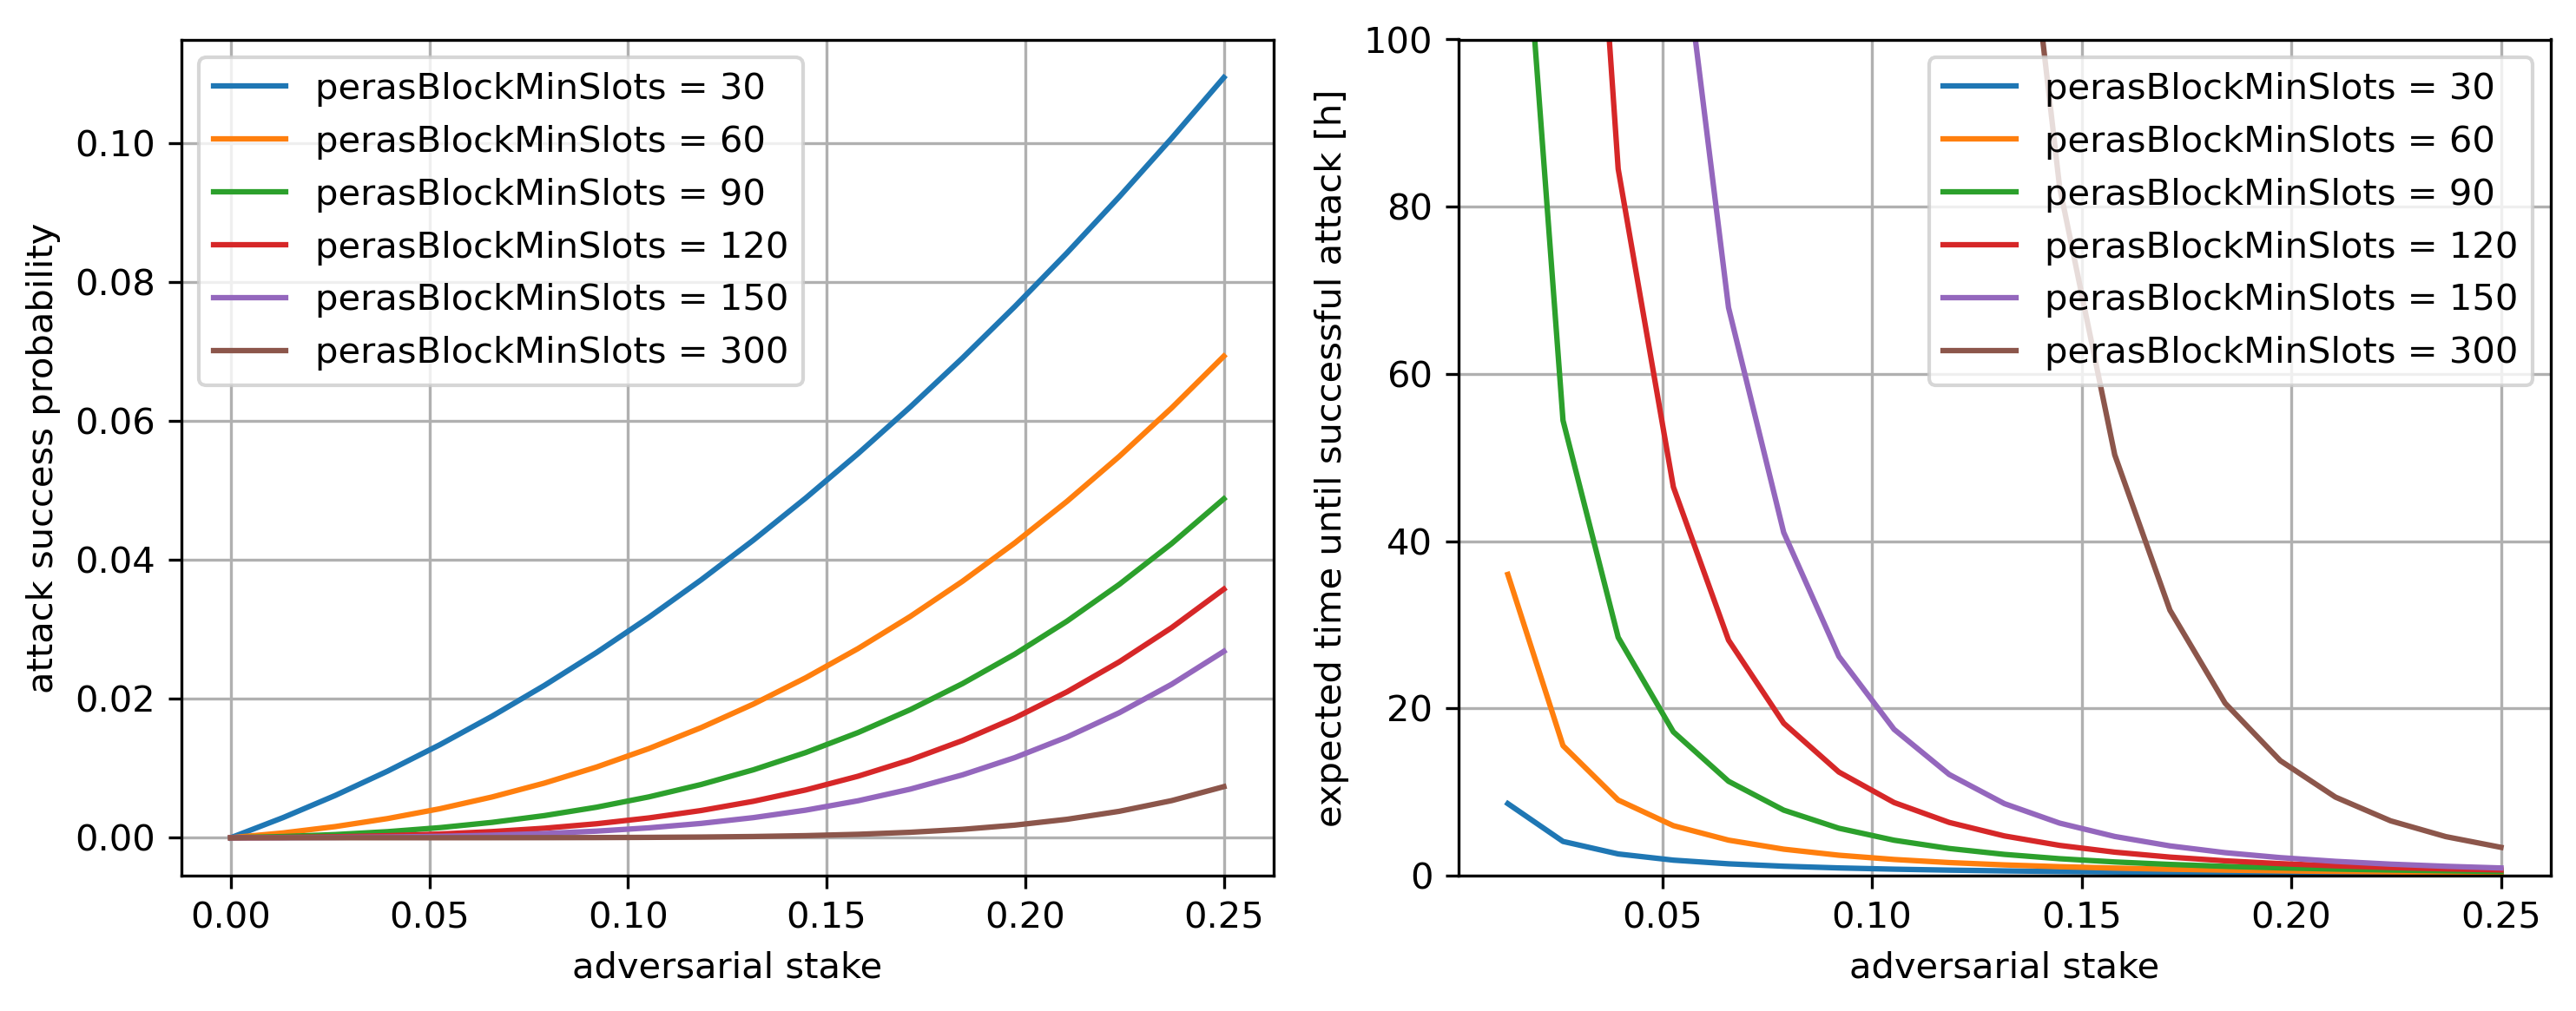
\includegraphics[width=0.95\textwidth]{./appendix/plot-honest-vote-splitting.png}
  \centering
  \caption{Probabilities (lower bounds) for \cref{lemma:honest vote splitting prob} for realistic parameters. The right plot assumes a slot length of one second and $\perasRoundSlots = 90$.}\label{fig:honest vote splitting prob}
\end{figure}
We plot the propabilities of \cref{lemma:honest vote splitting prob} for realistic parameters in \cref{fig:honest vote splitting prob}.
We observe that for small values for \perasBlockMinSlots{}, even relatively weak adversaries can execute a vote splitting attack rather frequently.
This is relevant in particular as it allows them to trigger a cooldown phase.

\subsection{Density reduction via boost-induced rollbacks}\label{sec:density reduction via boost-induced rollbacks}

We now describe an adversarial strategy that results in the honest historical chain to have low density, but high weight, i.e.\ in the extreme case, there is one boosted block per Peras round, with every voting round being successful.
In that case, a simple (private) fork purely made out of adversarial blocks has a good chance to have higher density (but significantly lower weight) than the honest chain.

See \cref{sec:weighted genesis} for how this attack influences the Peras design.

Consider a Peras round $r$ starting in slot $s$.
During round $r$, the adversary (with stake $\alpha$) does not diffuse any votes or blocks until shortly before the end of round $r$ in slot $s+\perasRoundSlots$.
Let $C$ be the best chain that any honest node has selected in slot $s+\perasRoundSlots-1$.
The adversary arranges it such that during the voting phase of round $r$, no quorum is reached without the adversarial votes, and further, that honest votes with weight at most $\perasQuorum - \alpha$ are cast for a block $B$ that is \emph{not} on $C$.
The idea now is for the adversary to diffuse its $\alpha\cdot\perasN$ votes for $B$ near the end of round $r$ such that round $r$ is considered successful and $B$ receives a boost.
Then, under reasonable assumptions, the chain ending in $B$ is preferrable to $C$ (as the latter doesn't contain a block that was boosted during round $r$), so the adversary succeeded in creating a low density but high weight chain during round $r$.

\medskip
Let us consider concretely how and under what conditions an attacker can execute this attack.
\begin{enumerate}
\item
  To start the attack, the attacker needs to prevent a quorum out of honest votes during round $r$, and needs to ensure that votes of weight at least $\perasQuorum - \alpha$ are cast for a block that the honest nodes will not build upon during round $r$.

  One way to accomplish this is to execute an honest vote splitting attack, see \cref{sec:honest vote splitting}.

  If $\alpha<0.25$, then the adversary must proceed exactly as described there, in particular, diffuse an appropriate chain right before round $r$ starts, in order to prevent a quorum purely made out of honest votes.
  On the other hande, if $\alpha\ge 0.25$, preventing an honest quorum is trivial, see \cref{sec:abstaining during voting}, so the adversary also has the option to diffuse the better chain even after $r$ started.
\item
  The round length \perasRoundSlots{} must not be too long in relation to \perasBoost{}, i.e.
  \[ \perasBoost \ge \phi(1-\alpha)\cdot \perasRoundSlots \;. \]
  Otherwise, the honest chain built during round $r$ might have more weight than the block $B$ (plus additional adversarial blocks on top of $B$) despite not having a boost.
  The attacker can still execute a less effective version of the attack by diffusing their votes signifcantly \emph{before} the end of round $r$.

  However, for realistic/useful Cardano mainnet parameters, such as $\perasRoundSlots = 90$ and $\perasBoost = 15$, this is not a problem for the adversary.
\item
  Once an adversary successfully performed the attack in a round, they can repeat it with good probability like this.
  The idea is for the adversary to mint two blocks $B_1,B_2$ on top of $B$ between slot $s-\perasBlockMinSlots$ and $s+\perasRoundSlots -\perasBlockMinSlots$, where $B_1$ is preferrable to $B_2$.
  Then, they execute an honest vote splitting attack between $B_1$ and $B_2$ for round $r+1$, such that neither block reaches quorum just due to honest votes, but such that $B_2$ votes having weight $\perasQuorum - \alpha$ at least.
  This is exactly the necessary setup to continue with the attack.

  The number of elections of a party with stake $\sigma$ within $n$ slots is given by
  \[ E_{n,\sigma}\sim\operatorname{Pois}(-n\sigma\log(1-\asc)) \]
  in the limiting case when the stake is distributed across infinitely many stake pools.
  Therefore, the probability that the adversary gets two elections in the aforementioned slot interval of size \perasRoundSlots{} is bounded by $P(E_{\perasRoundSlots,\alpha}\ge 2)$.
  For example, for $\perasRoundSlots = 90$ and $\alpha=0.4$, this evaluates to $55.09\%$.

  The number of successive successful rounds is hence geometrically distributed.
  Note that all blocks added to the chain in the meantime are adversarial, hence impacting chain quality.\footnote{However, such reductions in chain quality are not necessarily too unexpected in the presence of such strong adversaries, and the situation might overall still be better than with pure Praos.}
\end{enumerate}

These probabilities seem sufficiently large to us to take this attack seriously.
A more detailed analysis (potentially simulating the resulting Markov chain) is out-of-scope for this document.

\section{Attacks motivating aspects of the Peras design}

Here, we list attacks that motivate (and are hence prevented by) certain rules of the Peras design.

\subsection{Attack on a variant of the block creation rule}\label{sec:attack block creation rule}

Peras enters a \emph{cooldown period} when a round does not give rise to a certificate.
In order to coordinate the \emph{end} of the cooldown period, a certificate is included on chain.

When an honest node is elected in a slot in round $r$, it includes the latest certificate $\cert'$ it has seen if and only if all of the following hold:
\begin{enumerate}
\item\label{rule:block creation:a} The node has not seen a certificate $\cert$ with $\round(\cert)=r-2$.
\item\label{rule:block creation:b} $r-\round(\cert') \le \perasCertMaxSlots$.
\item\label{rule:block creation:c} $\round(\cert') > \round(\cert^*)$.
\end{enumerate}
Here, rule~\ref{rule:block creation:c} makes sure that an honest node never includes a certificate that has already been included in our current selection.
Rule~\ref{rule:block creation:b} allows us to disregard votes/certificates beyond a certain age.

Rule~\ref{rule:block creation:a} makes sure that all honest nodes have stopped voting, preventing useless certificate inclusions.
Concretely, rule~\ref{rule:block creation:a} implies that no honest node voted in round $r-1$, assuming that round $r-3$ was successful (i.e.\ we were not in a cooldown phase, so the voting rule (VR-2A) doesn't apply in round $r-1$).

To see this, we consider the contrapositive, i.e.\ assume that an honest node \emph{did} vote during round $r-1$.
Due to voting rule (VR-1A), it must have observed a certificate for round $r-2$ at the beginning of round $r-1$.
However, as $\perasRoundSlots\ge\perasDelta$, the votes for that certificate (including adversarial ones) must have been diffused to all honest nodes before round $r$.
Therefore, rule~\ref{rule:block creation:a} is not satisfied for any honest node during round $r$.\qed{}

In contrast, if we were to modify rule~\ref{rule:block creation:a} to be about the absence of a certificate in round $r-1$, then an adversary could force nodes to unnecessarily include a certificate on chain.
Concretely, the adversary can diffuse its votes shortly before the start of round $r$, such that some honest nodes see a quorum for round $r-1$, while others do not.
If the latter category of nodes is sufficiently small, then them not voting during round $r$ does not preclude the possibility of round $r$ being successful, in which case they will vote again in round $r$ as normal.
However, the modified rule~\ref{rule:block creation:a} would still force them to include the most recent certificate on chain when they are elected before they receive the adversarial votes for round $r-1$, which we want to avoid.

It may be useful to clarify that the harm of honest nodes unnecessarily including a certificate on chain is not necessarily the presence of the certificate itself.
Note that an adversary can include a certificate in any block they mint, for example, with the only risk being reputational harm.
Instead, the harm done by honest nodes including unnecessary certificates in the honest blocks they mint is that the limit on block size means the bytes occupied by the certificate could have otherwise been occupied by transactions.

\subsection{Adding weight to Genesis density comparisons}\label{sec:weighted genesis}

The implementation approach of Ouroboros Genesis in the Cardano node fundamentally relies on the following property, justified by the analysis of the Genesis chain selection rule in~\cite{badertscher2018ouroboros}:
\begin{tcolorbox}[title=\densityOfCompetingChainsName]\label{property:density-of-competing-chains}
  Let $p$ be any historical point on the honest chain. The honest chain of a net that has always executed Praos under nominal conditions will have strictly higher density in the \sgen{} slots immediately following $p$ than any alternative chain that intersects at $p$.
\end{tcolorbox}
Here, the \emph{density} of a chain in a range of slots is defined to be the number of blocks in that range.

\medskip
With Peras, it is natural to modify this property to talk about the \emph{weight} in the \sgen{} slots instead of just the number of blocks:
\begin{tcolorbox}[title=\weightedDensityOfCompetingChainsName]\label{property:weighted-density-of-competing-chains}
  Let $p$ be any historical point on the honest chain. The honest chain of a net that has always executed Peras under nominal conditions will have strictly higher weight in the \sgen{} slots immediately following $p$ than any alternative chain that intersects at $p$.
\end{tcolorbox}
In the implementation, relying on this rule instead of \densityOfCompetingChains{} results in additional complexity and operational costs:
\begin{itemize}
\item A syncing node must download certificates in order to perform Genesis density comparisons.
  This requires modifications to the existing Genesis logic, which currently gets by with looking purely at header chains.
\item Nodes need to store certificates boosting blocks on the historical/immutable chain stored indefinitely, such that they can be given to syncing peers.
  This increases disk and outbound bandwidth requirements.
\end{itemize}
However, this complexity is necessary, as \cref{sec:density reduction via boost-induced rollbacks} describes an attack that would be possible if we were to keep using \densityOfCompetingChains{} instead of implementing \weightedDensityOfCompetingChains{}.
Concretely, the adversary can use the attack to let the honest chain to have less than $\phi(\alpha) \cdot \sgen$ blocks (i.e.\ the average number of blocks on a chain they can create completely by themselves) in a window of $\sgen$ slots, despite having higher weight.
Once successful, the adversary can cause syncing nodes to commit to the adversarial chain permanently, violating safety.

\subsection{Spamming equivocating votes}\label{sec:attack equivocations}

The adversary can equivocate any of their seats in the voting committee of a Peras round by creating more than one vote for each seat, voting for different blocks.
An adversary with $\alpha<1/2$ stake can not use this to cause a quorum for different blocks in the same round due to the choice of $\perasQuorum = 3/4$ and a quorum intersection argument.

However, in a naive implementation, the adversary can use equivocating votes to cause unbounded additional network traffic for honest nodes.
Most directly, they can send many equivocating votes to any of their peers individually.
If this is disallowed (by requiring nodes to only forward the first vote per voting committee seat per round), the adversary can diffuse different equivocating votes to different peers, such that nodes still download many different equivocating votes from their peers.

We now describe how this can be avoided; specifically, honest nodes will only ever download at most one vote (or alternatively, a bounded amount of votes) per voting committee seat per round.

An honest node downloads votes from its peers in two stages:
\begin{enumerate}
\item\label{enumi:equivocation:step 1}
  In the first stage, it requests and downloads \emph{vote IDs} from its peers.

  The vote ID must be chosen as to uniquely identify a voting committee seat in a particular round.
  Concretely, it can be represented as the round number and a proof of eligibility, which might be the stake pool identity or a VRF proof.

  Also, we assume vote IDs to be significantly smaller than full votes.
\item\label{enumi:equivocation:step 2}
  In the second stage, the node downloads votes corresponding to all vote IDs \emph{without duplicates}.
  Upon receiving a vote, it is checked that the vote matches the supplied vote ID.\@

  This way, observing equivocating votes is impossible.
\end{enumerate}
As an optimization (for example to reduce the impact of slow peers), the same vote ID could also be requested from multiple peers (bounded by a small constant) in~\ref{enumi:equivocation:step 2}.
While possible and sound, it is not necessary to discard equivocating votes received this way.

Additionally, this approach requires us to diffuse of certificates in addition to votes in general (even between caught-up peers).
To see why, consider two honest nodes $H_1,H_2$ and an adversarial node $A$ which are pairwise connected.
Suppose that we are in round $r$, both $H_1$ and $H_2$ are only one vote short of a quorum for the block $B$ in round $r$, and all honest votes for round $r$ have already been diffused.
Now the adversary sends $H_1$ and $H_2$ a new vote ID $\mi{vid}$, and then equivocates $\mi{vid}$ to send a vote $v_B$ for $B$ to $A$, but a vote $v_{B'}$ for a block $B' \neq B$ to $A'$.
Now $A$ observes a quorum for $B$ in round $r$, creating a certificate, while $A'$ does not.
The vote diffusion mechanism described above causes $A'$ to not request a vote for $\mi{vid}$ from $A$, because $A'$ already has received $v_{B'}$.\footnote{Potentially, if $A'$ implements the optimization mentioned above, i.e.\ to download votes for the same vote id from multiple peers opportunistically, they might download $v_B$ from $A$, but this is not something we can rely on in general.}
Overall, the honest nodes $A$ and $A'$ now disagree whether round $r$ was successful, which they would not have if they had exchanged all equivocating votes.

However, by letting nodes also exchange \emph{certificates} in addition to votes, this scenario can be avoided.
Concretely, $A'$ would ask $A$ for a certificate for round $r$, and then download the certificate for $B$.
It does not matter that the certificate was built using an equivocating vote; in general, depending on the cryptographic scheme used for building certificates, it can even be impossible to detect this.
By construction, there can be at most one certificate per round, so there is no risk of equivocating certificates.



%%% Local Variables:
%%% mode: latex
%%% TeX-engine: xetex
%%% TeX-master: "../peras-design"
%%% End:


\end{document}

%%% Local Variables:
%%% TeX-engine: xetex
%%% End:
